\section{Simulation-based estimation}\label{sec:A-simulation}

The GMM and likelihood theory of \cref{sec:A-gmm,sec:A-mle} assumes that we can evaluate the moment function or the
density at any trial parameter. Many structural models in industrial organization imply moments or likelihoods that
are integrals with no closed form. The market share of a product in a random coefficients model integrates individual logit probabilities over
the distribution of tastes (\cref{ch:blp}). The expected winning bid in a first-price auction is the expected
second-highest value, an integral over the joint distribution of all bidders' values
\citep{LaffontOssardVuong1995}. The expected profit of an entrant integrates over values, rivals and bids
\citep{AtheyLevinSeira2011}. A counterfactual auction outcome is an expectation over simulated auctions
\citep{Asker2010}. This section shows how such integrals are replaced by averages over random draws and what the
replacement does to the properties of the estimator. The answer depends on how the simulated integral enters the
objective. When it enters linearly, as in a moment condition, simulation adds variance but no bias. When it enters
through a nonlinear function, such as a logarithm, it adds bias that vanishes only as the number of draws grows.

Throughout the section $\theta$ is a generic parameter vector, $n$ is the number of observations and $n_s$ is the
number of simulation draws per observation (the notation of \cref{ch:blp}). Several papers write $S$ for $n_s$, and
we translate their formulas.

\subsection{Monte Carlo integration}\label{sec:A-mc-integration}

Let $\nu$ be a random vector with known distribution $F$, which may depend on $\theta$ only through a known
transformation of standardized draws. The target is an expectation
\begin{equation}\label{eq:A-mc-target}
  \phi(\theta) = \E_\nu\bigl[q(\nu;\theta)\bigr] = \int q(\nu;\theta)\,\dd F(\nu),
\end{equation}
for a function $q$ that we can evaluate at any $(\nu, \theta)$. The \emph{Monte Carlo simulator} of $\phi(\theta)$
averages $q$ over $n_s$ independent draws $\nu_1, \dots, \nu_{n_s}$ from $F$:
\begin{equation}\label{eq:A-mc-simulator}
  \tilde\phi(\theta) = \frac{1}{n_s}\sum_{r=1}^{n_s} q(\nu_r;\theta).
\end{equation}

\begin{proposition}[Monte Carlo integration]\label{prop:A-mc}
Suppose $\sigma_q^2(\theta) = \Var_\nu(q(\nu;\theta))$ is finite. Then
\begin{enumerate}[label=(\roman*)]
  \item $\E[\tilde\phi(\theta)] = \phi(\theta)$, so the simulator is unbiased.
  \item $\Var(\tilde\phi(\theta)) = \frac{\sigma_q^2(\theta)}{n_s}$.
  \item $\sqrt{n_s}\,(\tilde\phi(\theta) - \phi(\theta)) \xrightarrow{d} N(0, \sigma_q^2(\theta))$ as $n_s \to \infty$.
\end{enumerate}
The simulation error is $O_p(n_s^{-\frac{1}{2}})$ whatever the dimension of $\nu$.
\end{proposition}

\begin{proof}
The draws are independent and identically distributed, so each term of \eqref{eq:A-mc-simulator} has mean
$\phi(\theta)$ and variance $\sigma_q^2(\theta)$. Linearity of expectation gives (i). Independence gives
\begin{equation*}
  \Var\bigl(\tilde\phi(\theta)\bigr) = \frac{1}{n_s^2}\sum_{r=1}^{n_s}\Var\bigl(q(\nu_r;\theta)\bigr)
  = \frac{n_s\,\sigma_q^2(\theta)}{n_s^2} = \frac{\sigma_q^2(\theta)}{n_s}.
\end{equation*}
Part (iii) is the Lindeberg-L\'evy central limit theorem. The dimension of $\nu$ enters only through
$\sigma_q^2$, which proves the last claim.
\end{proof}

The last statement explains why simulation dominates deterministic rules in high dimensions. A product quadrature
rule with $m$ nodes per dimension needs $m^d$ function evaluations in $d$ dimensions, while the accuracy of
\eqref{eq:A-mc-simulator} depends on $n_s$ alone. Quadrature and quasi-Monte Carlo sequences can be far more accurate
in one to three dimensions, and \cref{sec:08-quadrature} compares them for market shares.

\casehead{Uses in the book}
Four kinds of integrals recur. First, the random coefficients share $s_{jt} = \int s_{ijt}\,\dd F(\nu_i)$ is simulated
by averaging individual logit probabilities over draws of tastes (\cref{sec:08-simulation}). Second,
\citet{LaffontOssardVuong1995} simulate the expected winning bid of a first-price auction
(\cref{sec:A-snlls}). Third, \citet[p.~245]{AtheyLevinSeira2011} compute the expected profit of a logger or a mill
in a sealed-bid timber sale by simulation. They simulate 5,000 auctions for each plausible number of entering
loggers and mills, up to 8 mills and 25 loggers. Fourth, \citet{Asker2010} computes damages and efficiency losses from 100,000 auctions
simulated from estimated value distributions (\cref{sec:13-asker}).

\casehead{Smooth and frequency simulators}
When $q$ is an indicator, for example the indicator that a simulated consumer chooses product $j$, the simulator
\eqref{eq:A-mc-simulator} is a \emph{frequency simulator}. It is a step function of $\theta$ and can equal zero.
When part of the integral has a closed form, we can integrate it analytically and simulate only the rest. In logit
models the extreme value shocks are integrated exactly, and $q$ becomes a choice probability. The result is a
\emph{smooth simulator}. It is differentiable in $\theta$, strictly positive, and has smaller variance because
conditioning removes the variance of the integrated part (\cref{lem:08-smooth}).

\casehead{Common random numbers}
An estimator that uses simulated integrals evaluates them at many trial values of $\theta$. The draws must be taken
once, before estimation, and held fixed across all evaluations. With fresh draws at each evaluation the objective
function becomes a different random function every time it is computed. It is then discontinuous in $\theta$, and a
numerical optimizer never converges. With fixed draws the simulated objective is a single deterministic function
of $\theta$, so the draws can be treated as part of the data. Fixing the draws does not make that function smooth.
It is smooth when the simulator is smooth, while a frequency simulator remains a step function of $\theta$. The asymptotic theory below
treats the draws as part of the data. The practical rule ``take the draws only once'' is therefore part of the definition of the estimator.

\casehead{Importance sampling}
Draws from $F$ can be wasteful when $q$ is large only on a small region of the support. \emph{Importance sampling}
draws from another density $g$ and reweights. Let $f$ be the density of $\nu$ and write
\begin{equation*}
  \phi = \int q(\nu)\,f(\nu)\,\dd\nu = \int q(\nu)\,\frac{f(\nu)}{g(\nu)}\,g(\nu)\,\dd\nu
  = \E_g\Bigl[q(\nu)\,\frac{f(\nu)}{g(\nu)}\Bigr].
\end{equation*}
The ratio $w(\nu) = \frac{f(\nu)}{g(\nu)}$ is the \emph{importance weight}, and the importance sampling simulator is
\begin{equation}\label{eq:A-importance}
  \tilde\phi_g = \frac{1}{n_s}\sum_{r=1}^{n_s} q(\nu_r)\,w(\nu_r), \qquad \nu_r \overset{\text{i.i.d.}}{\sim} g.
\end{equation}

\begin{lemma}[Importance sampling]\label{lem:A-importance}
Suppose $g(\nu) > 0$ wherever $q(\nu)f(\nu) \ne 0$. Then
\begin{enumerate}[label=(\roman*)]
  \item $\E_g[\tilde\phi_g] = \phi$.
  \item $\Var_g(\tilde\phi_g) = \frac{1}{n_s}\Bigl[\int\frac{q(\nu)^2f(\nu)^2}{g(\nu)}\,\dd\nu - \phi^2\Bigr]$.
  \item The variance is minimized by $g^*(\nu) = \frac{|q(\nu)|f(\nu)}{\int|q(u)|f(u)\,\dd u}$. If $q \ge 0$, the
  minimum variance is zero.
\end{enumerate}
\end{lemma}

\begin{proof}
Part (i) is the change of measure displayed above. For (ii), each term has second moment
\begin{equation*}
  \E_g\bigl[q(\nu)^2w(\nu)^2\bigr] = \int q(\nu)^2\,\frac{f(\nu)^2}{g(\nu)^2}\,g(\nu)\,\dd\nu
  = \int\frac{q(\nu)^2f(\nu)^2}{g(\nu)}\,\dd\nu,
\end{equation*}
and its mean is $\phi$. Subtracting $\phi^2$ and dividing by $n_s$ gives (ii). For (iii), only the integral in (ii)
depends on $g$. The Cauchy-Schwarz inequality gives
\begin{equation*}
  \Bigl(\int|q|f\,\dd\nu\Bigr)^2 = \Bigl(\int\frac{|q|f}{\sqrt g}\,\sqrt g\,\dd\nu\Bigr)^2
  \le \int\frac{q^2f^2}{g}\,\dd\nu\cdot\int g\,\dd\nu = \int\frac{q^2f^2}{g}\,\dd\nu,
\end{equation*}
with equality when $\frac{|q|f}{\sqrt g}$ is proportional to $\sqrt g$, that is, when $g \propto |q|f$. If $q \ge 0$,
the bound equals $\phi^2$ and the variance in (ii) is zero.
\end{proof}

The optimal density $g^*$ is infeasible because its normalizing constant is $\phi$ itself. The lemma still guides
practice. A good importance density is close to proportional to $|q|f$. The variance in (ii) is finite exactly when
$\int\frac{q^2f^2}{g}\,\dd\nu < \infty$. This holds whenever the ratio $\frac{|q|f}{g}$ is bounded, since the integral
is then at most $\sup_\nu\frac{|q(\nu)|f(\nu)}{g(\nu)}\int|q|f\,\dd\nu$. A density $g$ with tails at least as heavy as
those of $|q|f$ is therefore the safe choice. Thinner tails can make the integral diverge, and then a few draws with
huge weights dominate the average. They need not do so. With $q = 1$, $f$ standard normal and $g$ normal with
variance $s^2$, the integral equals $\frac{s^2}{\sqrt{2s^2 - 1}}$, which is finite for every $s^2 > \frac{1}{2}$.
For $\frac{1}{2} < s^2 < 1$ the density $g$ has thinner tails than $f$, and the variance is still finite.
Importance sampling has a second advantage in estimation. If $\theta$ enters only through the weight
$\frac{f(\nu;\theta)}{g(\nu)}$ and the draws come from a fixed $g$, then the simulator is as smooth in $\theta$ as $f$.

Three applications in the book use it. \citet[pp.~960--961, 969]{LaffontOssardVuong1995} draw values from a
log-normal importance density centered at a preliminary estimate, and $\theta$ appears only in the density ratio
(\cref{sec:A-snlls}). \citet[p.~732, n.~31]{Gentzkow2007} draws each consumer's random effects from their
distribution conditional on the observed choices, computed at a preliminary estimate. That density is the posterior
of $\nu$ given the data, the analogue of $g^* \propto qf$ for a likelihood contribution. \citet[Section~6.3]{BerryLevinsohnPakes1995}
over-sample households likely to buy a new car, since most households buy none in a given year
(\cref{sec:08-importance}).

\begin{remark}[Sampling error versus simulation error]\label{rem:A-sampling-error}
Simulation error comes from the econometrician's draws and can be made small by raising $n_s$. Sampling error in
the data cannot. If an observed market share is the fraction of $M$ sampled consumers who buy a product, its
sampling standard deviation is about $\sqrt{\frac{s(1 - s)}{M}}$. In airline ticket samples with fewer than ten sampled
passengers per product, this error is large and is not removed by any number of simulation draws
(\cref{sec:09-bcs-estimation}). \Cref{sec:08-asymptotics} shows how \citet{BerryLevinsohnPakes1995} separate the
two sources in the asymptotic variance.
\end{remark}

\subsection{The method of simulated moments}\label{sec:A-msm}

The \emph{method of simulated moments} (MSM) of \citet{McFadden1989} and \citet{PakesPollard1989} replaces an
intractable conditional mean in a moment condition by an unbiased simulator. We state the leading case, a
conditional mean restriction. The data $w_i = (y_i, x_i)$ are i.i.d.\ across $i$, and
\begin{equation}\label{eq:A-msm-model}
  \E[y_i \mid x_i] = m(x_i;\theta_0), \qquad m(x;\theta) = \int q(x, \nu;\theta)\,\dd F(\nu).
\end{equation}
For example, $y_i$ may be a vector of choice indicators and $q$ the vector of logit probabilities given tastes
$\nu$. Let $z_i = z(x_i)$ be an $L \times \dim(y)$ matrix of instruments, functions of $x_i$. For each observation
we draw $\nu_{i1}, \dots, \nu_{in_s}$ from $F$, independently across $i$ and of the data, and form
\begin{equation}\label{eq:A-msm-sim}
  \tilde m_i(\theta) = \frac{1}{n_s}\sum_{r=1}^{n_s} q(x_i, \nu_{ir};\theta), \qquad
  \tilde g_n(\theta) = \frac{1}{n}\sum_{i=1}^{n} z_i\bigl(y_i - \tilde m_i(\theta)\bigr).
\end{equation}
The MSM estimator minimizes $\tilde g_n(\theta)^\top W_n\,\tilde g_n(\theta)$. Write $e_i = y_i - m(x_i;\theta_0)$
for the structural error and $\eta_i = \tilde m_i(\theta_0) - m(x_i;\theta_0)$ for the simulation error. Define
\begin{equation*}
  \Sigma_y(x) = \Var(y \mid x), \qquad V(x) = \Var_\nu\bigl(q(x, \nu;\theta_0)\bigr), \qquad
  G = -\E\Bigl[z_i\,\frac{\partial m(x_i;\theta_0)}{\partial\theta^\top}\Bigr].
\end{equation*}

\begin{proposition}[Method of simulated moments]\label{prop:A-msm}
Assume the conditions of \cref{thm:A-gmm-normal} for the GMM estimator with exact moments. Let $\nu$ be one draw from
$F$, independent of $(x_i, y_i)$, and let $\mathcal{N}$ be a closed neighborhood of $\theta_0$. Assume also that the
simulated moments satisfy the following conditions.
\begin{enumerate}[label=(\alph*)]
  \item $q(x, \nu;\theta)$ is continuous in $\theta$ on $\Theta$, and
  $\E\bigl[\sup_{\theta \in \Theta}\lVert z_i\,q(x_i, \nu;\theta)\rVert\bigr] < \infty$.
  \item $S_{\text{sim}} = \E[z_iV(x_i)z_i^\top]$ is finite.
  \item $q(x, \nu;\theta)$ is continuously differentiable in $\theta$ on $\mathcal{N}$, and
  $\E\bigl[\sup_{\theta \in \mathcal{N}}\bigl\lVert z_i\frac{\partial q(x_i, \nu;\theta)}{\partial\theta^\top}\bigr\rVert\bigr]
  < \infty$.
\end{enumerate}
Let $n_s$ be fixed and $W_n \xrightarrow{p} W$.
\begin{enumerate}[label=(\roman*)]
  \item The MSM estimator is consistent as $n \to \infty$.
  \item $\sqrt n(\hat\theta - \theta_0) \xrightarrow{d} N\bigl(0, (G^\top WG)^{-1}G^\top W\bigl[S + \tfrac{1}{n_s}S_{\text{sim}}\bigr]WG(G^\top WG)^{-1}\bigr)$,
  where $S = \E[z_i\Sigma_y(x_i)z_i^\top]$.
  \item If $V(x) \le \Sigma_y(x)$ for all $x$ in the positive semidefinite order, the asymptotic variance is at most
  $(1 + \frac{1}{n_s})$ times that of GMM with exact moments and the same $W$. The bound holds with equality for a
  frequency simulator of choice indicators.
\end{enumerate}
\end{proposition}

\begin{proof}
For (i), the summands of $\tilde g_n(\theta)$ are i.i.d.\ across $i$ because the data and the draws are. The simulator is
unbiased and the draws are independent of $y_i$, so $\E[\tilde m_i(\theta) \mid x_i, y_i] = m(x_i;\theta)$. Hence
\begin{equation*}
  \E\bigl[z_i(y_i - \tilde m_i(\theta))\bigr] = \E\bigl[z_i(y_i - m(x_i;\theta))\bigr]
  = \E\bigl[z_i\bigl(m(x_i;\theta_0) - m(x_i;\theta)\bigr)\bigr].
\end{equation*}
The population moment of the simulated estimator is the population moment of exact GMM. It is zero only at
$\theta_0$ by the identification condition. The uniform law of large numbers of \cref{lem:A-ulln} applies under
condition (a), and \cref{thm:A-consistency} gives consistency.

For (ii), evaluate the simulated moment at $\theta_0$:
\begin{equation*}
  \tilde g_n(\theta_0) = \frac{1}{n}\sum_{i=1}^{n} z_i\bigl[(y_i - m(x_i;\theta_0)) - (\tilde m_i(\theta_0) - m(x_i;\theta_0))\bigr]
  = \frac{1}{n}\sum_{i=1}^{n} z_i(e_i - \eta_i).
\end{equation*}
The summands are i.i.d.\ with mean zero. Conditional on $(x_i, y_i)$, $\eta_i$ has mean zero and variance
$\frac{1}{n_s}V(x_i)$ by \cref{prop:A-mc}, so $\E[z_i\eta_i\eta_i^\top z_i^\top] = \frac{1}{n_s}S_{\text{sim}}$, which is
finite by condition (b). The cross term vanishes:
\begin{equation*}
  \E\bigl[z_ie_i\eta_i^\top z_i^\top\bigr] = \E\bigl[z_ie_i\,\E[\eta_i \mid x_i, y_i]^\top z_i^\top\bigr] = 0.
\end{equation*}
Hence
\begin{equation*}
  \Var\bigl(z_i(e_i - \eta_i)\bigr) = \E[z_ie_ie_i^\top z_i^\top] + \E[z_i\eta_i\eta_i^\top z_i^\top]
  = S + \frac{1}{n_s}S_{\text{sim}},
\end{equation*}
and the Lindeberg-L\'evy central limit theorem gives $\sqrt n\,\tilde g_n(\theta_0) \xrightarrow{d} N(0, S +
\frac{1}{n_s}S_{\text{sim}})$. Condition (c) allows differentiation under the integral, so
$\E_\nu\bigl[\frac{\partial q}{\partial\theta^\top}\bigr] = \frac{\partial m}{\partial\theta^\top}$. The same
unbiasedness argument and \cref{lem:A-ulln}, applied on $\mathcal{N}$ to $z_i\frac{\partial q}{\partial\theta^\top}$,
show that the simulated Jacobian $\frac{\partial\tilde g_n}{\partial\theta^\top}$ converges uniformly to the exact one.
The mean value expansion in the proof of \cref{thm:A-gmm-normal} then applies unchanged.

For (iii), write
\begin{equation*}
  S + \frac{1}{n_s}S_{\text{sim}} = \Bigl(1 + \frac{1}{n_s}\Bigr)S - \frac{1}{n_s}\E\bigl[z_i(\Sigma_y(x_i) - V(x_i))z_i^\top\bigr].
\end{equation*}
The last expectation is positive semidefinite when $\Sigma_y \ge V$. Pre- and post-multiplying by
$(G^\top WG)^{-1}G^\top W$ and its transpose preserves the order. For a frequency simulator of a choice indicator,
$q$ is itself an indicator with $\Var_\nu(q \mid x) = \Sigma_y(x)$, so $V = \Sigma_y$.
\end{proof}

Condition (b) does not follow from the conditions for exact moments. Let $z_i = 1$, $y_i = \theta_0 + e_i$ with
$e_i$ standard normal, and $q(\nu;\theta) = \theta + \nu$ with $\nu$ a centered Student $t$ variable with 1.5 degrees
of freedom. Then $m(\theta) = \theta$, exact GMM satisfies \cref{thm:A-gmm-normal}, and conditions (a) and (c)
hold on a compact $\Theta$. The MSM estimator is
$\hat\theta = \bar y - \bar\nu$, with $\bar\nu$ the average of all $nn_s$ draws, and it is consistent. Since $\nu$ has
infinite variance, $\sqrt n(\hat\theta - \theta_0)$ has no normal limit. For simulated choice probabilities, $q$ lies in
$[0, 1]$, so the moment bounds in (a) and (b) hold whenever $\E\lVert z_i\rVert^2 < \infty$.

A frequency simulator is a step function of $\theta$, so it violates conditions (a) and (c). For such simulators,
\citet{PakesPollard1989} prove (i) and (ii) under \emph{stochastic equicontinuity}. This condition requires the
centered simulated moment $\tilde g_n(\theta) - \E[\tilde g_n(\theta)]$ to change by $o_p(n^{-\frac{1}{2}})$ over
shrinking neighborhoods of $\theta_0$. Smoothness is then needed only for the exact moment $m$, and the comparison in
(iii) applies unchanged.

The condition $V \le \Sigma_y$ holds for the smooth logit simulator. The smooth simulator is the conditional
expectation of the frequency simulator given the taste draw, so its variance is smaller by the law of total
variance (\cref{lem:08-smooth}). The factor $(1 + \frac{1}{n_s})$ is therefore an upper bound on the price of
simulation. With 10 draws per observation it is a 10 percent increase in variance, about 5 percent in standard
errors.

Two departures from the setting of the proposition are common in industrial organization. First, in market-level
demand estimation the draws are shared by all products in a market, and the number of markets or products drives
the asymptotics. The simulation error then adds a separate term to the variance of the moments, $V_3$ in
\citet{BerryLevinsohnPakes1995}. Their correction raised the reported standard errors by about 5 to 20 percent,
and one standard error doubled (p.~859, see \cref{sec:08-asymptotics}). Second, the simulated integral often enters
nonlinearly. The BLP inversion uses the logarithm of simulated shares, and $\E[\ln\tilde s] < \ln s$ by Jensen's
inequality. The bias is of order $\frac{1}{n_s}$ and does not average out across markets (\cref{prop:08-simbias}).
Consistency then requires $n_s$ to grow with the sample, exactly as for simulated maximum likelihood below.

MSM has two practical costs. Efficient MSM requires the optimal instruments of \cref{sec:A-optimal-iv}, which depend on
the unknown parameters and are computed from a preliminary estimate. When that estimate is poor, efficiency can be
poor as well \citep[pp.~43--44]{GourierouxMonfort1996}. In addition, moments for discrete outcomes require the
simulated probability of every possible outcome, which is expensive when the outcome space is large. Both points
led \citet[p.~732]{Gentzkow2007} to prefer simulated maximum likelihood.

\subsection{Simulated maximum likelihood}\label{sec:A-sml}

Let $(y_i, x_i)$ be i.i.d.\ across $i$, and let the density of $y_i$ given $x_i$ be a mixture over unobserved
heterogeneity,
\begin{equation*}
  f(y_i \mid x_i;\theta) = \int f(y_i \mid x_i, \nu;\theta)\,\dd F(\nu).
\end{equation*}
\emph{Simulated maximum likelihood} (SML), introduced by \citet{LermanManski1981}, maximizes
$\sum_i\ln\tilde f_i(\theta)$ with
\begin{equation}\label{eq:A-sml}
  \tilde f_i(\theta) = \frac{1}{n_s}\sum_{r=1}^{n_s} f_{ir}(\theta), \qquad
  f_{ir}(\theta) = f(y_i \mid x_i, \nu_{ir};\theta).
\end{equation}
The draws $\nu_{ir}$ come from $F$, independently across $i$ and $r$ and of the data. The simulator $\tilde f_i$ is
therefore unbiased for $f_i = f(y_i \mid x_i;\theta)$, but it enters through the logarithm.

\begin{proposition}[Bias of simulated maximum likelihood]\label{prop:A-sml-bias}
Let $v_i(\theta) = \Var_\nu(f(y_i \mid x_i, \nu;\theta))$, so that $\Var(\tilde f_i \mid x_i, y_i) =
\frac{v_i}{n_s}$. Assume the following.
\begin{enumerate}[label=(\alph*)]
  \item There are constants $0 < \underline{c} \le \bar c < \infty$ with $\underline{c} \le f(y \mid x, \nu;\theta) \le
  \bar c$ for all $(y, x, \nu, \theta)$. Choice probabilities satisfy the upper bound with $\bar c = 1$.
  \item $f(y \mid x, \nu;\theta)$ is twice continuously differentiable in $\theta$, with first and second derivatives
  bounded uniformly in $(y, x, \nu, \theta)$.
  \item $\Theta$ is compact, $\theta_0$ is interior and is the unique maximizer of $Q(\theta) = \E[\ln f_i(\theta)]$,
  and the Hessian $H$ of $Q$ at $\theta_0$ is nonsingular. For each $n_s$ the function $\E[\ln\tilde f_i(\theta)]$ has
  a unique maximizer $\theta_{n_s}$.
  \item The conditions of \cref{thm:A-mle-normal} hold for exact maximum likelihood.
\end{enumerate}
Then the following hold.
\begin{enumerate}[label=(\roman*)]
  \item Under (a), $\E\bigl[\ln\tilde f_i \mid x_i, y_i\bigr] = \ln f_i - \frac{1}{2}\,\frac{v_i}{n_sf_i^2} +
  O(n_s^{-\frac{3}{2}})$.
  \item Under (a) to (c), for fixed $n_s$ the SML estimator converges in probability to $\theta_{n_s}$. With
  $D(\theta) = \E\bigl[\frac{v_i(\theta)}{2f_i(\theta)^2}\bigr]$,
  $\theta_{n_s} - \theta_0 = \frac{1}{n_s}H^{-1}\nabla D(\theta_0) + o(\frac{1}{n_s})$ as $n_s \to \infty$. If
  $\nabla D(\theta_0) \ne 0$, then $\theta_{n_s} \ne \theta_0$ for all large $n_s$, and SML with any such fixed $n_s$
  is inconsistent.
  \item Under (a) to (d), if $n_s \to \infty$ and $\frac{\sqrt n}{n_s} \to 0$, then $\sqrt n(\hat\theta - \theta_0)
  \xrightarrow{d} N(0, \mathcal{I}^{-1})$, the limit of exact maximum likelihood.
\end{enumerate}
\end{proposition}

\begin{proof}
For (i), expand $\ln\tilde f_i$ around $f_i$ to third order with the Lagrange remainder:
\begin{equation*}
  \ln\tilde f_i = \ln f_i + \frac{\tilde f_i - f_i}{f_i} - \frac{(\tilde f_i - f_i)^2}{2f_i^2}
  + \frac{(\tilde f_i - f_i)^3}{3\bar f_i^3},
\end{equation*}
where $\bar f_i$ lies between $\tilde f_i$ and $f_i$, so $\bar f_i \ge \underline{c}$ by (a). The linear term has
conditional mean zero. The quadratic term has conditional mean $-\frac{v_i}{2n_sf_i^2}$. For the remainder, write
$\tilde f_i - f_i = \frac{1}{n_s}\sum_r d_r$ with $d_r = f_{ir} - f_i$. The $d_r$ are independent with mean zero and
$\lvert d_r\rvert \le \bar c$ by (a), so expanding the fourth power gives
\begin{equation*}
  \E\bigl[(\tilde f_i - f_i)^4 \mid x_i, y_i\bigr] = \frac{n_s\E[d_r^4] + 3n_s(n_s - 1)v_i^2}{n_s^4} \le
  \frac{3\bar c^4}{n_s^2}.
\end{equation*}
By Lyapunov's inequality the expected absolute cube is at most $(\frac{3\bar c^4}{n_s^2})^{\frac{3}{4}} =
O(n_s^{-\frac{3}{2}})$, so the expected absolute value of the remainder is at most this bound divided by $3\underline{c}^3$. The bound
holds uniformly in $i$ and $\theta$. The argument is the one in the proof of \cref{prop:08-simbias}.

For (ii), the simulated log-likelihood is an average of i.i.d.\ terms, each between $\ln\underline{c}$ and
$\ln\bar c$ and continuous in $\theta$. Their expectation is, by (i), $\E[\ln f_i(\theta)] - \frac{1}{n_s}D(\theta) +
O(n_s^{-\frac{3}{2}})$. By \cref{lem:A-ulln} and \cref{thm:A-consistency}, the extremum estimator converges to the
maximizer $\theta_{n_s}$ of this limit. As $n_s \to \infty$ the limit converges to $Q$ uniformly, so the argument of
\cref{thm:A-consistency} gives $\theta_{n_s} \to \theta_0$. Under (b), the same expansion applied to
$\nabla\ln\tilde f_i = \frac{\nabla\tilde f_i}{\tilde f_i}$ shows that the gradient of the remainder is also
$O(n_s^{-\frac{3}{2}})$, uniformly in $\theta$. The first-order condition at $\theta_{n_s}$ then reads
$\nabla Q(\theta_{n_s}) - \frac{1}{n_s}\nabla D(\theta_{n_s}) + O(n_s^{-\frac{3}{2}}) = 0$. A
first-order expansion of $\nabla Q$ around $\theta_0$, where $\nabla Q(\theta_0) = 0$, gives
\begin{equation*}
  H(\theta_{n_s} - \theta_0) = \frac{1}{n_s}\nabla D(\theta_0) + o\Bigl(\frac{1}{n_s}\Bigr), \qquad
  \theta_{n_s} - \theta_0 = \frac{1}{n_s}H^{-1}\nabla D(\theta_0) + o\Bigl(\frac{1}{n_s}\Bigr).
\end{equation*}
If $\nabla D(\theta_0) \ne 0$, the right side is nonzero for large $n_s$, so $\theta_{n_s} \ne \theta_0$. This is the
generic case, though not a universal one. If $f(y \mid x, \nu;\theta)$ does not depend on $\nu$, then $v_i = 0$, the
simulator is exact, and SML is maximum likelihood for every $n_s$.

For (iii) we sketch the argument of \citet{Lee1992} and \citet{GourierouxMonfort1996}. Decompose
\begin{equation*}
  \sqrt n(\hat\theta - \theta_0) = \sqrt n(\hat\theta - \theta_{n_s}) + \sqrt n(\theta_{n_s} - \theta_0).
\end{equation*}
By (ii) the second term is of order $\frac{\sqrt n}{n_s}$, which vanishes by assumption. The first term behaves like
the maximum likelihood estimator, plus a simulation variance of order $\frac{1}{n_s}$ that also vanishes.
\end{proof}

The proposition contrasts with \cref{prop:A-msm}. MSM is consistent with a single draw per observation. SML is in
general inconsistent for fixed $n_s$ by (ii), and under standard uniform regularity it is consistent when $n_s \to
\infty$ with $n$. Growth faster than $\sqrt n$ is the stronger condition of (iii). It removes the simulation bias at the $\sqrt n$
scale, so that SML attains the exact maximum likelihood limit. SML is nonetheless popular because it requires no
instruments, is efficient in the limit, and needs only the probability of the observed outcome.

\casehead{Bias correction}
Part (i) suggests removing the leading bias term. The sample variance of the $n_s$ terms in \eqref{eq:A-sml},
divided by $n_s$, is unbiased for $\Var(\tilde f_i)$:
\begin{equation*}
  \hat V_i = \frac{1}{n_s(n_s - 1)}\sum_{r=1}^{n_s}\bigl(f_{ir} - \tilde f_i\bigr)^2, \qquad
  \E\bigl[\hat V_i \mid x_i, y_i\bigr] = \frac{v_i}{n_s}.
\end{equation*}
The \emph{bias-corrected} SML estimator maximizes $\sum_i\bigl[\ln\tilde f_i + \frac{\hat V_i}{2\tilde f_i^2}\bigr]$
\citep[p.~45]{GourierouxMonfort1996}. Because $\hat V_i = O_p(\frac{1}{n_s})$ and $\tilde f_i = f_i +
O_p(n_s^{-\frac{1}{2}})$, the expectation of the correction equals $\frac{v_i}{2n_sf_i^2}$ up to
$O(n_s^{-\frac{3}{2}})$. The correction therefore removes the term of order $\frac{1}{n_s}$, and the remaining bias
is of smaller order.

\casehead{Evidence from a simulation}
\Cref{fig:A-simest} compares the estimators in a design where the integral is one-dimensional, so that exact
maximum likelihood can be computed by quadrature. Each of $N = 1{,}000$ individuals makes $T = 5$ binary choices with
utility $b_0 + \beta_ix_{it} + \epsilon_{it}$, logistic $\epsilon_{it}$, and a random coefficient $\beta_i \sim
N(b_1, \sigma^2)$ that is constant across the individual's choices. The true values are $b_0 = -0.5$ and $b_1 =
\sigma = 1$. The likelihood of individual $i$ integrates the product of five logit probabilities over $\beta_i$, as in
the partial panel of \citet{Gentzkow2007}. The MSM estimator uses three moments per individual. They match the
choice frequency, its covariance with $x_{it}$, and the frequency of repeated choices across pairs of occasions
weighted by $x_{it}x_{is}$. The last moment identifies $\sigma$, because a common $\beta_i$ makes choices persistent.

\begin{figure}[htbp]
\centering
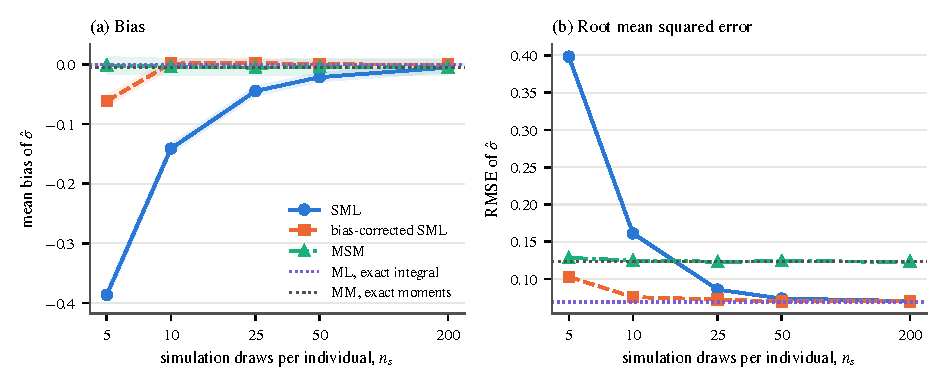
\includegraphics[width=\textwidth]{figures/appA/simest.pdf}
\caption{Simulation estimators of the standard deviation $\sigma$ of a random coefficient. Panel (a) shows the
mean bias of $\hat\sigma$ and panel (b) its root mean squared error, against the number of draws per individual.
The design is a panel binary logit with $N = 1{,}000$ individuals, $T = 5$ choices each, $x_{it} \sim N(0.5, 1)$,
$b_0 = -0.5$, $b_1 = 1$, $\sigma = 1$. SML uses \eqref{eq:A-sml}, bias-corrected SML adds
$\frac{\hat V_i}{2\tilde f_i^2}$, and MSM solves three simulated moment equations. The horizontal lines are maximum
likelihood and the exact-moment estimator computed with 40-point Gauss-Hermite quadrature. Shaded bands are
$\pm 1.96$ Monte Carlo standard errors. 300 replications, seed 20261022.}
\label{fig:A-simest}
\end{figure}

The results match the theory. With $n_s = 5$ draws, SML underestimates $\sigma = 1$ by 0.386 on average, and the
bias falls to 0.142, 0.045, 0.022 and 0.006 at 10, 25, 50 and 200 draws. From 25 draws on, $n_s$ times the bias is
roughly constant, as the $\frac{1}{n_s}$ rate predicts. The
bias pulls $\hat\sigma$ down because a smaller $\sigma$ makes the individual likelihood terms less variable across
draws, which raises $\E[\ln\tilde f_i]$ in part (i) of the proposition. The bias spills over to the mean coefficient
$b_1$, which is too small by 0.161 at five draws. The corrected estimator cuts the bias in $\hat\sigma$ to 0.062 at
five draws and to less than 0.003 from ten draws on. MSM is consistent at every fixed $n_s$, as \cref{prop:A-msm} predicts, and its Monte Carlo bias is small at every
$n_s$ in the table.
Its standard deviation at five draws is 0.129, against 0.123 with exact moments. The ratio of 1.04 is below the
bound $\sqrt{1 + \frac{1}{5}} = 1.10$ because the logit simulator is smooth. MSM's root mean squared error of about
0.12 exceeds that of maximum likelihood (0.069) at every $n_s$. Three just-identifying moments use the information
in the data less efficiently than the likelihood. SML overtakes MSM between 10 and 25 draws, and the corrected
version does so already at five.

\casehead{A worked case: Gentzkow (2007)}
\citet{Gentzkow2007} estimates a demand system for print and online newspapers in Washington, DC, from survey reports
of reading over the last day and the last five weekdays (\cref{sec:10-gentzkow}). The likelihood of a respondent's
report integrates a product of daily logit probabilities over a three-dimensional normal vector of random effects
(his eq.~6). He uses SML with 300 draws per consumer and the first-order bias correction of
\citet[p.~45]{GourierouxMonfort1996}. His footnote 32 derives the correction by the expansion in
\cref{prop:A-sml-bias}(i) (p.~732). The draws come from the importance density of \cref{lem:A-importance}. For each consumer he computes the
probability of the observed report once, at a preliminary estimate and with 200 draws. He then draws the random
effects from their distribution conditional on the report, by acceptance and rejection, and reweights
(p.~732, n.~31 and eqs.~13--14). Standard errors use the robust formula of \citet{McFaddenTrain2000}. Standard
errors of welfare statistics come from 100 draws from the estimated asymptotic distribution of the parameters
(p.~733), a method we discuss in \cref{sec:A-krinsky-robb}. He chose SML over MSM for the reasons given above. In
preliminary tests the two gave similar parameters, and MSM took 10 to 20 times longer to compute (p.~732). The
sample has 16,179 respondents (Table~5), large enough that the correction for $n_s = 300$ matters little, as in
\cref{fig:A-simest}. \Cref{sec:10-gentzkow-sml} gives the full estimator.

\subsection{Simulated nonlinear least squares}\label{sec:A-snlls}

\citet{LaffontOssardVuong1995} faced an integral inside a regression function. In a first-price or descending
auction with independent private values, the equilibrium bid function has no closed form for most value
distributions. The support of the winning bid also depends on the parameters. Maximum likelihood is then both
non-regular and computationally heavy, since the bid function must be inverted for every observation and every trial
parameter (p.~958, see \cref{prop:A-uniform-mle}). They proposed a least-squares estimator based on a simulated
conditional mean that is consistent for a fixed number of draws.

\casehead{The naive estimator and its limit}
Index auctions by $l = 1, \dots, n$ (their $L$), and let $b^w_l$ be the winning bid, with $b^w_l = p^o_l$ when the
object is unsold and $p^o_l$ the reserve price. Let $x_l$ collect the reserve price and the auction characteristics,
and let $m_l(\theta) = \E[b^w_l \mid x_l]$. Nonlinear least squares would minimize $\frac{1}{n}\sum_l(b^w_l -
m_l(\theta))^2$. Suppose $\bar X_l(\theta) = \frac{1}{n_s}\sum_{s=1}^{n_s}X_{sl}(\theta)$ is an unbiased simulator of
$m_l(\theta)$, with draws independent of $b^w_l$ given $x_l$. The naive estimator minimizes (their eq.~8)
\begin{equation}\label{eq:A-lov-naive}
  Q^{\text{naive}}_n(\theta) = \frac{1}{n}\sum_{l=1}^{n}\bigl(b^w_l - \bar X_l(\theta)\bigr)^2.
\end{equation}
To find its limit, write $b^w_l - \bar X_l(\theta) = (b^w_l - m_l(\theta_0)) + (m_l(\theta_0) - m_l(\theta)) +
(m_l(\theta) - \bar X_l(\theta))$. Given $x_l$, the first and third terms have mean zero and are independent of
each other, and the second is fixed. All cross products therefore have conditional mean zero, and
\begin{equation}\label{eq:A-lov-decomp}
  \E\bigl[(b^w_l - \bar X_l(\theta))^2 \mid x_l\bigr] = \sigma_0^2(x_l) + \bigl(m_l(\theta_0) - m_l(\theta)\bigr)^2
  + \frac{1}{n_s}\,\omega_l(\theta),
\end{equation}
where $\sigma_0^2(x_l) = \Var(b^w_l \mid x_l)$ and $\omega_l(\theta) = \Var(X_{sl}(\theta) \mid x_l)$. The first term
does not depend on $\theta$, and the second is minimized at $\theta_0$. The third term is the average simulator
variance, $A_L(\theta)$ in their eq.~(9). It depends on $\theta$, so the naive estimator converges to a value that
trades fit for a smaller simulator variance. It is inconsistent for fixed $n_s$ whenever the gradient of the
average simulator variance is nonzero at $\theta_0$, which is the generic case.

\casehead{The corrected estimator}
The sample variance of the draws, divided by $n_s$, is unbiased for $\frac{1}{n_s}\omega_l(\theta)$. Subtracting it
gives the simulated nonlinear least squares (SNLLS) objective (their eqs.~10--11):
\begin{equation}\label{eq:A-lov-snlls}
  Q^*_n(\theta) = \frac{1}{n}\sum_{l=1}^{n}\Bigl[\bigl(b^w_l - \bar X_l(\theta)\bigr)^2
  - \frac{1}{n_s(n_s - 1)}\sum_{s=1}^{n_s}\bigl(X_{sl}(\theta) - \bar X_l(\theta)\bigr)^2\Bigr].
\end{equation}
By \eqref{eq:A-lov-decomp}, each bracket has conditional mean $\sigma_0^2(x_l) + (m_l(\theta_0) - m_l(\theta))^2$, the
limit of exact nonlinear least squares. The estimator is consistent for any fixed $n_s$ as $n \to \infty$ (their
Proposition~1), and $Q^*_n(\hat\theta)$ consistently estimates the mean squared error of the model.

Its asymptotic variance shows the price of simulation (their Proposition~2). Let $\mu_l = \frac{\partial
m_l(\theta_0)}{\partial\theta}$, let $Y_{sl}(\theta) = \frac{\partial X_{sl}(\theta)}{\partial\theta}$, and let
$\omega_l$, $\Omega_l$ and $C_l$ be the conditional variances of $X_{sl}(\theta_0)$ and $Y_{sl}(\theta_0)$ and their
covariance. Then $\sqrt n(\hat\theta - \theta_0) \xrightarrow{d} N(0, \mathcal{H}^{-1}\mathcal{J}\mathcal{H}^{-1})$ with
$\mathcal{H} = \E[\mu_l\mu_l^\top]$ and
\begin{equation}\label{eq:A-lov-avar}
  \mathcal{J} = \E\Bigl[\sigma_0^2(x_l)\mu_l\mu_l^\top + \frac{1}{n_s}\bigl(\sigma_0^2(x_l)\Omega_l + \omega_l\mu_l\mu_l^\top\bigr)
  + \frac{1}{n_s(n_s - 1)}\bigl(\omega_l\Omega_l + C_lC_l^\top\bigr)\Bigr].
\end{equation}
The first term alone gives the variance of exact nonlinear least squares. The excess is of order $\frac{1}{n_s}$
and disappears as $n_s \to \infty$. Their Proposition~3 gives a heteroskedasticity-robust estimator of
$\mathcal{H}^{-1}\mathcal{J}\mathcal{H}^{-1}$ that is also consistent for fixed $n_s$.

\casehead{The simulator: revenue equivalence}
The construction of $X_{sl}$ uses auction theory. Let $N$ bidders (their $I$) have independent values from $F_l(\cdot;\theta)$
with density $f_l$, and let $v_{(N)}$ and $v_{(N-1)}$ be the highest and second-highest values. For a value $v \ge
p^o$, the first-price equilibrium bid equals the expected payment of the winner in a second-price auction (their
Lemma, eq.~12):
\begin{equation*}
  e(v) = \E\bigl[\max(v_{(N-1)}, p^o) \mid v_{(N)} = v\bigr].
\end{equation*}
The winning bid is $e(v_{(N)})$ when the object sells, and the convention $b^w = p^o$ covers the unsold case. Taking
expectations over $v_{(N)}$ with the law of iterated expectations gives (their eq.~14)
\begin{equation*}
  m_l(\theta) = \E\bigl[\max(v_{(N-1)l}, p^o_l)\bigr]
  = \int\!\!\cdots\!\!\int\max\bigl(u_{(N-1)}, p^o_l\bigr)\prod_{i=1}^{N}f_l(u_i;\theta)\,\dd u_1\cdots\dd u_N.
\end{equation*}
This is the revenue equivalence theorem at work: the expected winning bid equals the expected second-highest value,
truncated at the reserve price (\cref{ch:auction-theory}). The integrand needs no bid function. With importance
densities $g_l$ and draws $u^s_{1l}, \dots, u^s_{Nl}$ from $g_l$, the simulator is (their eq.~17)
\begin{equation*}
  X_{sl}(\theta) = \max\bigl(u^s_{(N-1)l}, p^o_l\bigr)\prod_{i=1}^{N}\frac{f_l(u^s_{il};\theta)}{g_l(u^s_{il})}.
\end{equation*}
The parameter appears only in the density ratio outside the maximum, so $Q^*_n$ is twice continuously
differentiable when $f_l$ is. Simulating with draws from $F_l(\cdot;\theta)$ would instead put $\theta$ inside the
maximum. With draws $F_l^{-1}(U^s_{il};\theta)$ from fixed uniforms $U^s_{il}$, the maximum is continuous in $\theta$ but
kinked where the reserve starts to bind. A frequency simulator built from indicators of simulated events would be a
step function of $\theta$. Neither would make $Q^*_n$ twice continuously differentiable.

\casehead{The application}
The data are 81 descending auctions of greenhouse eggplants in Marmande, France, in the summer of 1990, each selling
a single case (p.~967). Values are log-normal, with the mean of log values linear in six auction characteristics and
the standard deviation fixed at 0.05 from retail price dispersion (pp.~968--969). The estimates use 20 draws per
auction, and 30 draws gave analogous results (p.~969, n.~19). The number of bidders is treated as an unknown integer.
The criterion is minimized over $N$ from 11, the number of regular buyers, to 23, and the minimum is at $N = 18$
(p.~970). This suggests that one large buyer acts for about eight retailers. The fit gives an $R^2$ of 0.895 (p.~971).
\Cref{ch:auction-empirics} discusses the estimates.

\subsection{Indirect inference}\label{sec:A-indirect}

\emph{Indirect inference} \citep{GourierouxMonfortRenault1993,Smith1993} fits a simple auxiliary model to the real
data and to data simulated from the structural model. It chooses $\theta$ so that the two fits agree. Let
$\hat\beta$ be an auxiliary estimator, such as OLS coefficients or the parameters of a reduced-form logit, computed
on the data. For a trial $\theta$, simulate $H$ data sets of the same size from the structural model with fixed
draws, compute $\tilde\beta_h(\theta)$ on each, and average them into $\bar\beta(\theta)$. The estimator is
\begin{equation*}
  \hat\theta = \argmin_\theta\bigl(\hat\beta - \bar\beta(\theta)\bigr)^\top W\bigl(\hat\beta - \bar\beta(\theta)\bigr).
\end{equation*}
The probability limit of $\tilde\beta_h(\theta)$ is the \emph{binding function} $b(\theta)$, and identification
requires $b$ to be one to one near $\theta_0$. The auxiliary model need not be correctly specified. If
$\sqrt n(\hat\beta - b(\theta_0))$ has asymptotic variance $\Lambda$, the $H$ independent simulated estimates have
the same variance each, so the average has variance $\frac{\Lambda}{H}$. The estimator therefore behaves like a
minimum-distance estimator with variance inflated by the factor $(1 + \frac{1}{H})$, the analogue of
\cref{prop:A-msm}. MSM is the special case in which the auxiliary statistics are sample moments.

\subsection{Inference on functions of estimated parameters}\label{sec:A-krinsky-robb}

Many reported quantities are nonlinear functions $a(\theta)$ that are themselves computed by simulation: median
margins, welfare changes, predicted auction outcomes. The delta method of \cref{sec:A-delta} needs the derivative of
$a$, which may be costly or unstable. \citet{KrinskyRobb1986} proposed a simulation alternative.

\begin{remark}[Drawing from the estimated asymptotic distribution]\label{rem:A-krinsky-robb}
Given $\hat\theta$ and an estimate $\hat V$ of its variance:
\begin{enumerate}[label=(\arabic*)]
  \item Draw $\theta^{(1)}, \dots, \theta^{(R)}$ independently from $N(\hat\theta, \hat V)$.
  \item Compute $a(\theta^{(r)})$ for each draw, solving any equilibrium or simulation problem that $a$ requires.
  \item Report the standard deviation of the $a(\theta^{(r)})$, or their 2.5 and 97.5 percentiles as a 95 percent
  interval.
\end{enumerate}
\end{remark}

The method is common in the book's applications. \citet[Table~VIII, note]{Nevo2001} computes 95 percent intervals
for median margins from 1,500 draws (\cref{sec:08-nevo01}). \citet[p.~733]{Gentzkow2007} uses 100 draws for welfare
statistics. \citet[p.~248]{AtheyLevinSeira2011} call their version a parametric bootstrap. They resample from the
asymptotic distribution of the bid and entry parameters and recompute the expected auction outcomes for each draw.

The method rests on the same approximation as the delta method, the normality of $\hat\theta$. It retains the
nonlinearity of $a$, which helps when $a$ is far from linear over the likely range of $\theta$. It does not correct a
poor normal approximation for $\hat\theta$ itself, and it does not resample the data. \Cref{sec:A-boot-multistep}
compares it with bootstraps that re-estimate the model.

\section{Standard errors under dependence}\label{sec:A-se}

The variance formulas of \cref{sec:A-ols,sec:A-gmm} assume independent observations. Industrial organization data
rarely satisfy that assumption. Prices of the same product are observed in many cities, products in the same market
share demand shocks, and a state's prices are observed every year. This section derives the cost of ignoring such
dependence and the estimators that allow for it.

\subsection{One formula for all robust variances}\label{sec:A-se-meat}

Consider the linear model $y = X\beta + e$ with $n$ observations and $K$ regressors, and the OLS estimator
$\hat\beta = (X^\top X)^{-1}X^\top y$. Its sampling error is $\hat\beta - \beta = (X^\top X)^{-1}\sum_i x_ie_i$, so
conditional on $X$
\begin{equation}\label{eq:A-sandwich-general}
  \Var(\hat\beta \mid X) = (X^\top X)^{-1}\,\Omega_n\,(X^\top X)^{-1}, \qquad
  \Omega_n = \sum_{i=1}^{n}\sum_{j=1}^{n}x_ix_j^\top\E[e_ie_j \mid X].
\end{equation}
Every robust variance estimator replaces the ``meat'' $\Omega_n$ by
\begin{equation}\label{eq:A-meat-kernel}
  \hat\Omega_n = \sum_{i=1}^{n}\sum_{j=1}^{n}k_{ij}\,x_ix_j^\top\hat e_i\hat e_j,
\end{equation}
for weights $k_{ij} \in [0, 1]$ that state which pairs of observations may be correlated. The estimators differ only
in $k_{ij}$:
\begin{itemize}
  \item Heteroskedasticity-robust estimators (HC, \citealp{White1980}) set $k_{ij} = \indic\{i = j\}$.
  \item Cluster-robust estimators set $k_{ij} = \indic\{c(i) = c(j)\}$, with $c(i)$ the cluster of observation $i$.
  \item The Newey-West estimator for a time series sets $k_{ij} = \max\{0, 1 - \frac{|t_i - t_j|}{m+1}\}$ for a lag
  length $m$.
  \item Two-way clustering sets $k_{ij} = \indic\{g(i) = g(j) \text{ or } h(i) = h(j)\}$ for two grouping variables.
  \item Spatial HAC estimators \citep{Conley1999} let $k_{ij}$ decline in the economic distance between $i$ and $j$.
\end{itemize}
Plugging $\hat e_i\hat e_j$ for $e_ie_j$ is useless for a single pair, but the sum over many pairs averages out the
noise. Each estimator is consistent when the pairs it drops are uncorrelated and the pairs it keeps are few relative
to the sample. \Cref{sec:A-ols-asy} covered the HC case, including the finite-sample versions HC1 to HC3. HC estimators
suffice when observations are independent. The rest of this section treats the other cases.

\subsection{Clustered data}\label{sec:A-cluster}

Let the observations fall into $C$ clusters, $c = 1, \dots, C$, with $n_c$ observations in cluster $c$. Errors are
independent across clusters and may be correlated within. We first measure the cost of ignoring the correlation.

\begin{proposition}[Moulton factor]\label{prop:A-moulton}
Let $y_{ic} = \alpha + \beta x_{ic} + e_{ic}$ with $C$ clusters of equal size $\bar n$. Conditional on the
regressor, let the errors be homoskedastic with variance $\sigma^2$, uncorrelated across clusters and equicorrelated
within clusters with correlation $\rho_e$. Let $\tilde x_{ic} = x_{ic} - \bar x$ and define the intra-cluster
correlation of the regressor as
\begin{equation*}
  \rho_x = \frac{\sum_{c}\sum_{i \ne j}\tilde x_{ic}\tilde x_{jc}}{(\bar n - 1)\sum_c\sum_i\tilde x_{ic}^2}.
\end{equation*}
Then
\begin{equation}\label{eq:A-moulton}
  \Var(\hat\beta \mid x) = \frac{\sigma^2}{\sum_c\sum_i\tilde x_{ic}^2}\,\bigl[1 + (\bar n - 1)\rho_x\rho_e\bigr].
\end{equation}
The first factor is the conventional OLS variance. If the regressor is constant within clusters, $\rho_x = 1$ and the
factor is $1 + (\bar n - 1)\rho_e$.
\end{proposition}

\begin{proof}
By the Frisch-Waugh-Lovell theorem, $\hat\beta - \beta = \frac{\sum_c\sum_i\tilde x_{ic}e_{ic}}{\sum_c\sum_i\tilde
x_{ic}^2}$. Write $D = \sum_c\sum_i\tilde x_{ic}^2$. The numerator has variance
\begin{align*}
  \Var\Bigl(\sum_c\sum_i\tilde x_{ic}e_{ic}\Bigr)
  &= \sum_c\Bigl[\sum_i\tilde x_{ic}^2\sigma^2 + \sum_{i \ne j}\tilde x_{ic}\tilde x_{jc}\rho_e\sigma^2\Bigr] \\
  &= \sigma^2D + \rho_e\sigma^2(\bar n - 1)\rho_xD \\
  &= \sigma^2D\,\bigl[1 + (\bar n - 1)\rho_x\rho_e\bigr].
\end{align*}
The first line uses independence across clusters and the equicorrelation within. The second substitutes the
definition of $\rho_x$. Dividing by $D^2$ gives \eqref{eq:A-moulton}. If $x$ is constant within clusters, every
cross product $\tilde x_{ic}\tilde x_{jc}$ equals $\tilde x_{ic}^2$, so the numerator of $\rho_x$ is $(\bar n - 1)D$.
\end{proof}

The factor can be large even when $\rho_e$ is modest. With 20 observations per cluster and $\rho_x = \rho_e = 0.5$,
it equals $1 + 19 \times 0.25 = 5.75$, so the true standard error is $\sqrt{5.75} = 2.40$ times the conventional one.
A nominal 5 percent $t$-test that uses the conventional standard error then rejects a true null with probability
about $\Pr(|Z| > \frac{1.96}{2.40}) = 0.41$ in large samples. With unequal cluster sizes, \citet{Moulton1986} shows
that $\bar n - 1$ is replaced by $\frac{\Var(n_c)}{\bar n} + \bar n - 1$. \citet{Moulton1990} documents the problem
for regressions of individual outcomes on aggregate variables, where $\rho_x = 1$.

\casehead{The cluster-robust variance}
The cluster-robust estimator of \citet{LiangZeger1986} sets $k_{ij} = \indic\{c(i) = c(j)\}$ in
\eqref{eq:A-meat-kernel}. With $X_c$ and $\hat e_c$ the rows of cluster $c$, and the finite-sample factor used by
most software, it is
\begin{equation}\label{eq:A-cr1}
  \hat V_{\text{CR1}} = \frac{C}{C - 1}\,\frac{n - 1}{n - K}\,(X^\top X)^{-1}\Bigl(\sum_{c=1}^{C}X_c^\top\hat e_c\hat e_c^\top
  X_c\Bigr)(X^\top X)^{-1}.
\end{equation}
It allows any correlation and heteroskedasticity within clusters. Its consistency rests on the number of clusters.
When cluster sizes are bounded and $C \to \infty$, the terms $X_c^\top e_ce_c^\top X_c$ are independent across
clusters, and $\frac{1}{C}\sum_cX_c^\top e_ce_c^\top X_c$ converges to its mean by a law of large numbers.
Replacing $e_c$ by $\hat e_c$ changes the average by $o_p(1)$ because $\hat\beta$ is consistent. When each
observation is its own cluster, $C = n$ and $\frac{C}{C - 1}\frac{n - 1}{n - K} = \frac{n}{n - K}$, so CR1 reduces
to HC1. For 2SLS, replace $X$ by $\hat X = P_ZX$ in the bread and $x_i\hat e_i$ by $\hat x_i\hat e_i$ in the meat,
with residuals computed from $X$. For GMM, estimate the long-run covariance of the moments by
$\hat S = \frac{1}{n}\sum_c\hat g_c\hat g_c^\top$ with $\hat g_c = \sum_{i \in c}g(w_i;\hat\theta)$. When fixed
effects are nested within clusters, software differs on whether $K$ counts them. We count every regressor,
including the dummies, which gives slightly larger standard errors.

\casehead{The level of clustering}
The cluster should contain every pair of observations whose errors may be correlated, and clusters must be
numerous. \citet{BertrandDufloMullainathan2004} show the stakes for difference-in-differences regressions on
state-year panels.\footnote{We read NBER Working Paper 8841 (2002), the working-paper version of
\citet{BertrandDufloMullainathan2004}. Pages marked WP refer to it.} Placebo state laws, assigned at random, were
``significant'' at the 5 percent level in up to 45 percent of their simulations with conventional standard errors
(WP p.~3). Outcomes and treatment indicators are both serially correlated within states. Clustering by state, the
level at which treatment is assigned, restored approximately correct size with many states. The rejection rate was
6 percent in their panel of 51 states, and it rose to 8.5 percent with 10 states and 15 percent with 6 states (WP p.~18 and Table~9).
\citet{AbadieEtAl2023} add a design-based view. Clustering adjusts for
clustered sampling or clustered assignment of the regressor of interest. Correlated outcomes alone do not call for it
when assignment is at the individual level and the sample covers the population.

\casehead{Two-way clustering}
In a state-year panel, errors may be correlated within states over time and within years across states. Two-way
clustering \citep{CameronGelbachMiller2011} keeps every pair that shares a state or a year. The indicator of that
event satisfies the inclusion-exclusion identity
\begin{equation*}
  \indic\{g(i) = g(j) \text{ or } h(i) = h(j)\} = \indic\{g(i) = g(j)\} + \indic\{h(i) = h(j)\}
  - \indic\{g(i) = g(j),\ h(i) = h(j)\}.
\end{equation*}
Substituting into \eqref{eq:A-meat-kernel} gives $\hat V_{\text{2way}} = \hat V_g + \hat V_h - \hat V_{g \cap h}$:
cluster by the first dimension, cluster by the second, and subtract the estimate clustered by their intersection. In a
panel with one observation per state-year, the intersection estimator is the HC estimator. The difference can fail to
be positive semidefinite in small samples, and then negative eigenvalues are set to zero. Asymptotic justification
requires the number of clusters in both dimensions to grow, so inference should use the smaller of the two counts.

\casehead{Few clusters}
With few clusters, CR1 standard errors are too small and $t$-statistics are far from normal. Two corrections are
standard \citep{CameronMiller2015}. The first compares the $t$-statistic with the quantiles of the $t$ distribution
with $C - 1$ degrees of freedom. The second is the wild cluster bootstrap of \citet{CameronGelbachMiller2008}.

\begin{remark}[Wild cluster bootstrap-$t$]\label{rem:A-wild-cluster}
To test $H_0: \beta_k = \beta_k^0$ with CR1 standard errors:
\begin{enumerate}[label=(\arabic*)]
  \item Compute $t = \frac{\hat\beta_k - \beta_k^0}{\widehat{\mathrm{se}}_{\text{CR1}}(\hat\beta_k)}$ from the data.
  \item Estimate the model with the null imposed, and keep its coefficients $\tilde\beta$ and residuals $\tilde e_{ic}$.
  \item For $b = 1, \dots, B$, draw one weight $w_c^{(b)} \in \{-1, 1\}$ per cluster, each value with probability
  $\frac{1}{2}$ (Rademacher weights), and form $y^{(b)}_{ic} = x_{ic}^\top\tilde\beta + w_c^{(b)}\tilde e_{ic}$.
  \item Regress $y^{(b)}$ on $X$, and compute $t^{(b)} = \frac{\hat\beta^{(b)}_k -
  \beta_k^0}{\widehat{\mathrm{se}}_{\text{CR1}}(\hat\beta^{(b)}_k)}$ with the same formula as in step (1).
  \item Report the $p$-value $\frac{1}{B}\sum_{b=1}^{B}\indic\{|t^{(b)}| \ge |t|\}$. Count as ties the values of
  $|t^{(b)}|$ that differ from $|t|$ only by rounding error. If $2^C \le B$, use all $2^C$ weight vectors in place
  of random draws, and set $B = 2^C$.
\end{enumerate}
\end{remark}

Three features make the procedure work. Multiplying a whole cluster's residuals by one weight preserves any
correlation pattern within the cluster. Imposing the null makes the bootstrap data satisfy the hypothesis being
tested, which improves size. The statistic is studentized, which yields the asymptotic refinement of
\cref{sec:A-boot}.

When very few clusters are treated, the residuals of treated clusters carry the treatment effect estimate and the wild
bootstrap fails \citep{MacKinnonWebb2017}. Methods that use the control clusters to estimate the error
distribution are then needed \citep{ConleyTaber2011}.

\casehead{Discreteness with Rademacher weights}
With Rademacher weights there are only $2^C$ weight vectors, each with probability $2^{-C}$. The vectors $w$ and
$-w$ give bootstrap estimates $\hat\beta^{(b)}_k - \beta^0_k$ of opposite sign and residuals of opposite sign, so
they give the same $|t^{(b)}|$. Hence $|t^{(b)}|$ takes at most $2^{C-1}$ distinct values \citep{CameronMiller2015}.
The vector of ones reproduces the data, so it and its negative give $|t^{(b)}| = |t|$ exactly. The \emph{exact
conditional bootstrap $p$-value} is the probability of $|t^{(b)}| \ge |t|$ over all $2^C$ vectors, given the data.
It is at least $\frac{2}{2^C}$, which equals $\frac{1}{16} = 0.0625$ when $C = 5$. A 5 percent test with five clusters
therefore never rejects. The $p$-value of step (5) with random draws is a simulation estimate of the exact
$p$-value. It can fall below $\frac{2}{2^C}$ when few draws hit the two tying vectors, and enumeration removes this
noise. Rounding error can also make a computed $|t^{(b)}|$ fall just below $|t|$ for a tying vector, which is why
step (5) counts ties explicitly. Weight distributions with more support points make the $p$-value finer.
With fewer than ten clusters, \citet{CameronMiller2015} recommend the six-point weights of \citet{Webb2013}. These put probability
$\frac{1}{6}$ on each of $\pm\sqrt{\frac{1}{2}}$, $\pm 1$ and $\pm\sqrt{\frac{3}{2}}$, which have mean zero and
variance one.

\begin{figure}[htbp]
\centering
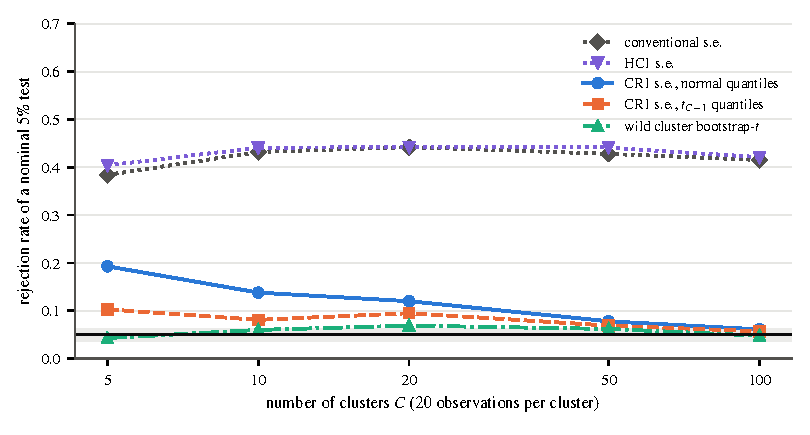
\includegraphics[width=0.86\textwidth]{figures/appA/cluster_mc.pdf}
\caption{Rejection rates of nominal 5 percent tests of a true null when errors and the regressor are both
correlated within clusters. In the design, $y_{ic} = e_{ic}$ is regressed on a constant and $x_{ic}$. Both $x_{ic}$
and $e_{ic}$ are sums of independent normal cluster and idiosyncratic components, with intra-cluster correlations
$\rho_x = \rho_e = 0.5$. There are 20 observations per cluster and 1,000 replications per $C$, with seed 20261022.
With $C = 5$ the Rademacher bootstrap enumerates all 32 weight vectors. The six-point bootstrap uses 399 random
weight vectors for every $C$, and the Rademacher bootstrap does so for $C \ge 10$. The gray band is the 95 percent Monte Carlo range around 0.05.}
\label{fig:A-cluster-mc}
\end{figure}

\Cref{fig:A-cluster-mc} reports a simulation with the parameters of the Moulton example. The conventional test
rejects the true null in 38 to 44 percent of replications for every number of clusters, close to the 41 percent
predicted above. HC1 standard errors do no better, because the problem is correlation, which HC1 ignores.
CR1 standard errors with normal quantiles reject 19 percent of the time with 5 clusters, 14 percent with 10 and 6
percent with 100. Using $t_{C-1}$ quantiles lowers the rejection rate to 10 percent with 5 clusters and 8 to 10
percent with 10 to 20 clusters. With Rademacher weights and at least 10 clusters, the wild cluster bootstrap rejects
between 4.8 and 6.9 percent of the time. With 5 clusters it never rejects, because its exact $p$-value is at least
0.0625 in every replication. A $p$-value simulated from 399 random draws would reject in 1.0 percent of the
replications with ties counted, and in 4.3 percent if rounding error drops the ties. The near-nominal second
figure is an artifact of the tie comparison. The six-point weights reject between 4.8 and 7.5 percent of the time
for every $C$, and 5.6 percent with 5 clusters. Each rate has a Monte Carlo standard error of about 0.007.

\subsection{Serial correlation and HAC estimators}\label{sec:A-hac}

In a time series $t = 1, \dots, T$, let $g_t$ be a mean-zero score or moment, for example $x_te_t$. Write
$\Gamma_j = \E[g_tg_{t-j}^\top]$ for its autocovariance at lag $j$, with $\Gamma_{-j} = \Gamma_j^\top$. Under
covariance stationarity,
\begin{equation*}
  \Var\Bigl(\frac{1}{\sqrt T}\sum_{t=1}^{T}g_t\Bigr) = \frac{1}{T}\sum_{t=1}^{T}\sum_{s=1}^{T}\Gamma_{t-s}
  = \sum_{j=-(T-1)}^{T-1}\Bigl(1 - \frac{|j|}{T}\Bigr)\Gamma_j \longrightarrow S = \sum_{j=-\infty}^{\infty}\Gamma_j,
\end{equation*}
where the middle step counts the $T - |j|$ pairs with $t - s = j$ and the limit holds when the autocovariances are
absolutely summable. The matrix $S$ is the \emph{long-run variance}. With $g_t = x_te_t$ and $n = T$, the meat
$\Omega_n$ of \eqref{eq:A-sandwich-general} is the variance of $\sum_tg_t$, which is approximately $TS$. An estimate
$\hat S$ therefore enters the OLS sandwich as $\hat\Omega_n = T\hat S$:
\begin{equation*}
  \widehat\Var(\hat\beta) = (X^\top X)^{-1}\,T\hat S\,(X^\top X)^{-1} = \frac{1}{T}\,\hat Q^{-1}\hat S\hat Q^{-1},
  \qquad \hat Q = \frac{X^\top X}{T}.
\end{equation*}
In the GMM formulas, $\hat S$ replaces $S$ directly.

\begin{example}[AR(1) regressor and error]\label{ex:A-ar1-factor}
Let $x_t$ and $e_t$ be independent stationary AR(1) processes with autocorrelations $\rho_x$ and $\rho_e$. Then
$\Gamma_j = \E[x_tx_{t-j}]\E[e_te_{t-j}] = \sigma_x^2\sigma_e^2(\rho_x\rho_e)^{|j|}$, and
\begin{equation*}
  S = \sigma_x^2\sigma_e^2\Bigl[1 + 2\sum_{j=1}^{\infty}(\rho_x\rho_e)^j\Bigr]
  = \sigma_x^2\sigma_e^2\,\frac{1 + \rho_x\rho_e}{1 - \rho_x\rho_e}.
\end{equation*}
The conventional variance uses only $\Gamma_0 = \sigma_x^2\sigma_e^2$, so it is too small by the factor
$\frac{1 + \rho_x\rho_e}{1 - \rho_x\rho_e}$. With $\rho_x = 0.85$ and $\rho_e = 0.64$, the factor is 3.4 and the
standard error ratio is 1.8. These are the within-state autocorrelations of the tax and of the residual in the
cigarette panel of \cref{sec:A-sumner-se}.
\end{example}

\casehead{The Newey-West estimator}
A natural estimator truncates the sum at lag $m$ and uses sample autocovariances
$\hat\Gamma_j = \frac{1}{T}\sum_{t=j+1}^{T}\hat g_t\hat g_{t-j}^\top$. The unweighted truncated sum can fail to be
positive semidefinite. \citet{NeweyWest1987} downweight the autocovariances linearly:
\begin{equation}\label{eq:A-newey-west}
  \hat S_{\text{NW}} = \hat\Gamma_0 + \sum_{j=1}^{m}\Bigl(1 - \frac{j}{m+1}\Bigr)\bigl(\hat\Gamma_j + \hat\Gamma_j^\top\bigr).
\end{equation}
The Bartlett weights $1 - \frac{j}{m+1}$ guarantee a positive semidefinite estimate. To see why, form the block sums
$\hat B_t = \sum_{k=0}^{m}\hat g_{t-k}$ and consider $\frac{1}{(m+1)T}\sum_t\hat B_t\hat B_t^\top$, an average of
outer products and hence positive semidefinite. Expanding the product, $\hat g_{t-k}\hat g_{t-l}^\top$ appears for
each pair $(k, l)$, and the number of pairs with $k - l = j$ is $m + 1 - |j|$. The weight on lag $j$ is therefore
$\frac{m + 1 - |j|}{m+1} = 1 - \frac{|j|}{m+1}$, which reproduces \eqref{eq:A-newey-west} up to terms at the ends
of the sample. Consistency requires $m \to \infty$ with $\frac{m}{T} \to 0$. A common rule of thumb is $m =
\lfloor 4(\frac{T}{100})^{\frac{2}{9}}\rfloor$. In \citet[p.~634]{NeweyWest1994} this formula is only a preliminary
lag in an automatic procedure for the Bartlett kernel. The procedure uses it to estimate a constant $\hat\gamma$ and then
sets $m = \lfloor\hat\gamma T^{\frac{1}{3}}\rfloor$ (p.~635).
\citet{GenesoveMullin1998} report Newey-West standard errors with four lags for their quarterly sugar demand and
pricing equations (\cref{sec:03-sugar}).

\casehead{Panels}
In a panel with many units and a short time dimension, clustering by unit allows arbitrary serial correlation
within units, and nothing more is needed if units are independent. When units share common shocks that time
effects do not remove, \citet{DriscollKraay1998} average the scores across units within each period and apply
\eqref{eq:A-newey-west} to the resulting time series. Their estimator allows any cross-sectional dependence, but it
requires a long panel and allows only serial correlation that dies out within $m$ periods. \citet{Conley1999}
extends the HAC idea to dependence that declines with spatial or economic distance.

\subsection{Dependence structures in IO data}\label{sec:A-io-dependence}

The book's applications show four recurring structures. The first is the same product observed in many markets in
the same period, whose prices respond to common cost and demand shocks.
\citet[WP p.~25]{AshenfelterHosken2010} observe the prices of the same products in many geographic markets each
period,\footnote{We read NBER Working Paper 13859 (2008) of \citet{AshenfelterHosken2010} and NBER Working Paper
17476 (2011) of \citet{AshenfelterHoskenWeinberg2013}. Pages marked WP refer to them.} and therefore cluster on the time period, citing \citet{Moulton1987}. Their reference list contains only
\citet{Moulton1990} (WP p.~39), which makes the same point about aggregate regressors. The second is the same product or
unit observed repeatedly over time. \citet[WP p.~14]{AshenfelterHoskenWeinberg2013} cluster by SKU in their
appliance price regressions. \citet[pp.~862--863]{BerryLevinsohnPakes1995} treat the sum of the moments of a car model over
all its years as one observation, which allows any correlation across years for a given model. The third is common
shocks to all products in a market. \citet[WP p.~17]{BerryCarnallSpiller1996} assume independence across airline
markets and a factor structure that correlates demand and cost errors within a market (\cref{sec:09-bcs-estimation}).
They also note that the average product has fewer than 10 sampled passengers, and they leave the correction of
standard errors for this sampling error to future research (WP p.~17). The fourth
is serial correlation that a structural model must represent explicitly. \citet{Ellison1994} models an AR(1) demand
error inside his Markov-switching likelihood, and doing so changes the point estimates as well as the standard
errors (\cref{ch:collusion-evidence}). \Cref{tab:A-se-practice} collects the inference methods used in the book.

\begin{table}[htbp]
\centering
\begin{threeparttable}
\caption{Inference under dependence in the book's applications}
\label{tab:A-se-practice}
\footnotesize
\begin{tabularx}{\textwidth}{@{}>{\raggedright\arraybackslash}p{2.7cm}>{\raggedright\arraybackslash}X>{\raggedright\arraybackslash}X>{\raggedright\arraybackslash}p{2.6cm}@{}}
\toprule
Application & Data structure & Inference used & Source \\
\midrule
\citet{Sumner1981}, re-estimated & State-year panel, 48 units, 25 years & Clusters by state, by year and both, Driscoll-Kraay, wild cluster bootstrap & \Cref{tab:A-sumner} \\
\addlinespace
\citet{GenesoveMullin1998} & Quarterly time series, 1890--1914 & Newey-West, 4 lags, with the pricing equation corrected for estimated demand & \Cref{sec:03-sugar} \\
\addlinespace
\citet{AshenfelterHosken2010} & Product by city by period & Clusters on the time period & WP p.~25 \\
\addlinespace
\citet{AshenfelterHoskenWeinberg2013} & SKU by month & Clusters by SKU & WP p.~14 \\
\addlinespace
\citet{BerryLevinsohnPakes1995} & Car model by year & Moments summed over a model's years, simulation variance added & pp.~862--863 and \cref{sec:08-asymptotics} \\
\addlinespace
\citet{BerryCarnallSpiller1996} & Products in airline markets & Independence across markets and a factor structure within them, share sampling error not corrected & WP p.~17 and \cref{sec:09-bcs-estimation} \\
\addlinespace
\citet{MillerWeinberg2017} & Brand-size product by region by period & Clusters by region, two-step correction for estimated demand & pp.~1775, 1780 and \cref{ch:mergers} \\
\addlinespace
\citet{ChaudhuriGoldbergJia2006} & Product by region by month & Bootstrap over months, 300 replications, all products and regions kept & WP p.~21 \\
\addlinespace
\citet{Nevo2001} & Brand by city by quarter & 1,500 draws from the asymptotic distribution for median margins & Table~VIII \\
\addlinespace
\citet{Asker2010} & Auctions & Bootstrap over auctions, 5,000 iterations, 90 percent intervals & Tables~7--10 \\
\addlinespace
\citet{Gentzkow2007} & Survey respondents & Robust SML standard errors, 100 parameter draws for welfare & p.~733 \\
\addlinespace
\citet{AtheyLevinSeira2011} & Timber sales & Matching standard errors of \citet{AbadieImbens2006}, parametric bootstrap & pp.~230, 248 \\
\bottomrule
\end{tabularx}
\begin{tablenotes}\footnotesize
\item Notes: WP page numbers refer to working-paper versions of the papers.
\end{tablenotes}
\end{threeparttable}
\end{table}

\subsection{Worked application: Sumner's regression revisited}\label{sec:A-sumner-se}

\citet{Sumner1981} tests for competition in cigarettes by regressing the retail price per pack on the excise tax in a
state-year panel (\cref{sec:A-panel,sec:03-sumner-design}). His most complete specification is the two-way fixed effects
regression \eqref{eq:A-sumner} of \cref{sec:A-panel},
\begin{equation*}
  p_{sy} = \mu_s + \tau_y + \rho\,t_{sy} + e_{sy},
\end{equation*}
with state effects $\mu_s$, year effects $\tau_y$ and pass-through $\rho$. Competition with flat marginal cost
implies $\rho = 1$. Sumner reports $\hat\rho = 1.074$ with a conventional standard error of 0.013 (Table~1), so the
$t$-statistic for $\rho = 1$ is 5.7. Both the price and the tax are persistent within states, so the
conventional standard error is suspect.

We re-estimate the regression on a panel reconstructed from \emph{The Tax Burden on Tobacco} (1983, Table~13) and
the CPI-U of the Bureau of Labor Statistics. It covers 47 states and the District of Columbia from 1954 to 1978,
1,200 state-years, the same coverage as Sumner's. Prices and taxes are nominal cents per pack, and the tax is the
state tax plus the federal tax of 8 cents. The computations are in \texttt{figures/appA/src/sumner\_inference.py}.
\Cref{tab:A-sumner} reports three specifications and six variance estimators.

\begin{table}[htbp]
\centering
\begin{threeparttable}
\caption{Cigarette tax pass-through: standard errors and tests of $\rho = 1$ under different dependence assumptions}
\label{tab:A-sumner}
\small
\setlength{\tabcolsep}{3.6pt}
\begin{tabular}{@{}lccccccccc@{}}
\toprule
& Sumner & \multicolumn{8}{c}{Re-estimation} \\
\cmidrule(lr){2-2}\cmidrule(l){3-10}
Specification & (1981) & $\hat\rho$ & Conv. & HC1 & State & Year & Two-way & DK & Wild \\
\midrule
(1) State, year effects, OLS & \makecell{1.074\\(0.013)} & 1.075 & 0.013 & 0.015 & 0.034 & 0.013 & 0.033 & 0.016 & \\
\quad $p$-value for $\rho = 1$ & & & $<$0.001 & $<$0.001 & 0.033 & $<$0.001 & 0.034 & $<$0.001 & 0.044 \\
\addlinespace
(2) CPI, OLS & \makecell{1.029\\(0.011)} & 1.029 & 0.011 & 0.013 & 0.030 & 0.023 & 0.035 & 0.027 & \\
\quad $p$-value for $\rho = 1$ & & & 0.007 & 0.030 & 0.340 & 0.207 & 0.416 & 0.299 & 0.358 \\
\addlinespace
(3) CPI, random effects & \makecell{1.069\\(0.013)} & 1.069 & 0.013 & 0.015 & 0.033 & 0.015 & 0.033 & 0.020 & \\
\quad $p$-value for $\rho = 1$ & & & $<$0.001 & $<$0.001 & 0.042 & $<$0.001 & 0.046 & 0.002 & \\
\bottomrule
\end{tabular}
\begin{tablenotes}\footnotesize
\item Notes: The dependent variable is the retail price in cents per pack and the regressor of interest the combined
state and federal tax in cents per pack, 1,200 state-years. The first column reproduces Sumner's Table~1 (standard
errors in parentheses). The other columns report our estimate of $\rho$ and its standard error under six
estimators. Conv.: conventional OLS or GLS. HC1: heteroskedasticity-robust. State and Year: CR1 clustered by state
(48 clusters) or by year (25). Two-way: clustered by state and year \citep{CameronGelbachMiller2011}. DK:
\citet{DriscollKraay1998} with Bartlett weights and 2 lags. $p$-values use normal quantiles for Conv.\ and HC1,
$t_{47}$ for State, $t_{24}$ for Year, Two-way and DK. Wild: wild cluster bootstrap-$t$ by state with the null
imposed, Rademacher weights and 9,999 draws. Row (2) replaces the year effects by the national CPI and drops the
state effects. Row (3) has the regressors of row (2) and is two-way random-effects GLS \citep{FullerBattese1974}, and
its robust variants apply the formulas to the GLS-transformed regression. $K$ counts all dummies in row (1).
\end{tablenotes}
\end{threeparttable}
\end{table}

\casehead{Row (1)}
The re-estimation reproduces Sumner's estimate and conventional standard error. The HC1 standard error is 15
percent larger. Clustering by state raises the standard error to 0.034, 2.6 times the conventional value. The
within-state first-order autocorrelation of the residuals is 0.64 and that of the within-transformed tax is 0.85.
\Cref{ex:A-ar1-factor} predicts a standard error ratio of about 1.8 for these values, and the ratio of the clustered to
the HC1 standard error is 2.2. Clustering by year leaves the standard error at 0.013. The year effects absorb the
common national shocks, so the residuals of different states in the same year are nearly uncorrelated. The two-way
estimate, 0.033, is close to the state-clustered one for the same reason. The Driscoll-Kraay estimate, 0.016, allows
any correlation across states but only two lags of serial correlation, and it misses the persistence that clustering
by state captures. The rejection of $\rho = 1$ survives every estimator that allows correlation within states, with
$p$-values from 0.033 to 0.044, but its margin is far thinner than a $t$-statistic of 5.7 suggests. The wild cluster
bootstrap $p$-value of 0.044 has a Monte Carlo standard error of 0.002.

\casehead{Row (2)}
Without state effects, persistent differences in state price levels enter the error, and they are correlated over
time within a state. The conventional standard error of 0.011 gives $p = 0.007$. Clustering by state, by year or by both, the
Driscoll-Kraay estimator and the wild cluster bootstrap all give $p$ above 0.2. The apparent rejection of competition in this specification is an
artifact of the conventional standard error.

\casehead{Row (3)}
The random-effects GLS estimate reproduces Sumner's 1.069. Its conventional standard error assumes that a constant
state effect captures all within-state correlation. The residuals of the transformed regression remain serially
correlated, and the state-clustered standard error is 0.033, with $p = 0.042$. Random effects therefore do not
substitute for clustering when the error has more persistence than a permanent effect.

The lesson is general. In a panel with persistent regressors and errors, the conventional and heteroskedasticity-robust
standard errors can overstate precision by a factor of two or more. The clustering level should follow the
dependence that the fixed effects leave in the error. Here the fixed effects leave serial correlation within
states, while the correlation across states within a year is negligible.

\section{The delta method and the bootstrap}\label{sec:A-delta-boot}

Empirical work rarely stops at the estimated parameters. A pass-through coefficient is turned into an elasticity,
demand parameters into markups, and a demand system into the welfare effect of a counterfactual. This section
develops the two general tools for the uncertainty of such quantities, the delta method and the bootstrap, and
shows when each fails.

\subsection{The delta method}\label{sec:A-delta}

\begin{theorem}[Delta method]\label{thm:A-delta}
Suppose $\sqrt n(\hat\theta - \theta_0) \xrightarrow{d} N(0, V)$ for $\theta_0 \in \R^K$. Let $a: \R^K \to \R^q$ be
continuously differentiable in a neighborhood of $\theta_0$, with Jacobian $A(\theta) = \frac{\partial
a(\theta)}{\partial\theta^\top}$ ($q \times K$) and $A = A(\theta_0)$. Then
\begin{equation*}
  \sqrt n\bigl(a(\hat\theta) - a(\theta_0)\bigr) \xrightarrow{d} N(0, AVA^\top).
\end{equation*}
If $\hat V \xrightarrow{p} V$, then $A(\hat\theta)\hat VA(\hat\theta)^\top \xrightarrow{p} AVA^\top$.
\end{theorem}

\begin{proof}
Since $\sqrt n(\hat\theta - \theta_0)$ converges in distribution, $\hat\theta - \theta_0 = O_p(n^{-\frac{1}{2}})$ and
$\hat\theta \xrightarrow{p} \theta_0$. For each component $a_k$, the mean value theorem gives a point $\bar\theta_k$
on the segment between $\hat\theta$ and $\theta_0$ with
\begin{equation*}
  a_k(\hat\theta) - a_k(\theta_0) = \frac{\partial a_k(\bar\theta_k)}{\partial\theta^\top}(\hat\theta - \theta_0).
\end{equation*}
Stack these rows into a matrix $\bar A$. Each $\bar\theta_k \xrightarrow{p} \theta_0$, so $\bar A \xrightarrow{p} A$
by continuity of the derivatives. Then
\begin{equation*}
  \sqrt n\bigl(a(\hat\theta) - a(\theta_0)\bigr) = \bar A\,\sqrt n(\hat\theta - \theta_0),
\end{equation*}
and Slutsky's theorem gives convergence to $A\,N(0, V) = N(0, AVA^\top)$. The second claim follows from the
continuous mapping theorem.
\end{proof}

In practice the delta-method standard error of a scalar $a(\hat\theta)$ is $\sqrt{\nabla a(\hat\theta)^\top\hat
V_n\nabla a(\hat\theta)}$, where $\hat V_n = \frac{\hat V}{n}$ is the estimated variance of $\hat\theta$. We now work
through the cases that recur in the book.

\begin{example}[Elasticity implied by pass-through]\label{ex:A-delta-passthrough}
Under monopoly or constant conduct with constant-elasticity demand and flat marginal cost, pass-through is $\rho =
\frac{\varepsilon}{\varepsilon - 1}$, where $\varepsilon$ is the elasticity the firms behave as if they face
(\cref{sec:03-sumner-design}). Inverting gives $\varepsilon = a(\rho) = \frac{\rho}{\rho - 1}$ for $\rho > 1$. The
derivative is
\begin{equation*}
  a'(\rho) = \frac{(\rho - 1) - \rho}{(\rho - 1)^2} = -\frac{1}{(\rho - 1)^2},
  \qquad \mathrm{se}(\hat\varepsilon) = \frac{\mathrm{se}(\hat\rho)}{(\hat\rho - 1)^2}.
\end{equation*}
Sumner's estimate $\hat\rho = 1.074$ with standard error 0.013 gives $\hat\varepsilon = \frac{1.074}{0.074} = 14.5$ and
a delta-method standard error of $\frac{0.013}{0.074^2} = 2.37$.\footnote{Sumner's printed implied elasticities equal
$\frac{1}{1 - \hat\rho}$, for example $-13.5$ for the first row. They are one unit smaller in magnitude than
$\frac{\hat\rho}{\hat\rho - 1}$, because they treat $\hat\rho - 1$ as the markup over cost instead of using the Lerner
condition (\cref{sec:03-sumner-design}).} Our re-estimate $\hat\rho = 1.0746$ gives $\hat\varepsilon = 14.4$, with a
standard error of 2.38 based on the conventional standard error and 6.11 based on the state-clustered one. The
standard error of $\hat\varepsilon$ is about 180 times that of $\hat\rho$, because the derivative is the inverse
square of $\hat\rho - 1 = 0.075$.
\end{example}

\begin{example}[Marginal cost from an inverse-elasticity rule]\label{ex:A-delta-cost}
With an observed price $p$ and an estimated elasticity, the Lerner rule $\frac{p - c}{p} = \frac{1}{\varepsilon}$
gives $\hat c = p(1 - \frac{1}{\hat\varepsilon})$ (\cref{prop:01-infer-cost}). The derivative
$\frac{\dd c}{\dd\varepsilon} = \frac{p}{\varepsilon^2}$ yields $\mathrm{se}(\hat c) = \frac{p}{\hat\varepsilon^2}
\mathrm{se}(\hat\varepsilon)$. Chaining with \cref{ex:A-delta-passthrough}, $c = p(1 - \frac{\rho - 1}{\rho}) =
\frac{p}{\rho}$, so $\mathrm{se}(\hat c) = \frac{p}{\hat\rho^2}\mathrm{se}(\hat\rho)$. The cost implied by
pass-through is precise even when the elasticity is not, because a markup of a few percent is small whatever its
exact value.
\end{example}

\begin{example}[Willingness to pay as a ratio]\label{ex:A-delta-ratio}
In a demand model with utility $x\beta - \alpha p$, the willingness to pay for characteristic $k$ is $r =
\frac{\beta_k}{\alpha}$. The gradient with respect to $(\beta_k, \alpha)$ is $(\frac{1}{\alpha}, -\frac{\beta_k}
{\alpha^2})$, so
\begin{equation*}
  \widehat{\Var}(\hat r) = \frac{1}{\hat\alpha^2}\Bigl[\hat V_{kk} - 2\hat r\hat V_{k\alpha} + \hat r^2\hat V_{\alpha\alpha}\Bigr],
\end{equation*}
with $\hat V$ the estimated covariance of $(\hat\beta_k, \hat\alpha)$. When $\hat\alpha$ is imprecise, the
distribution of the ratio is far from normal. \citet{Fieller1954} proposed an exact alternative under normality.
The statistic $\hat\beta_k - r\hat\alpha$ has mean zero at the true ratio and variance $V_{kk} - 2rV_{k\alpha} +
r^2V_{\alpha\alpha}$. The Fieller set collects the values $r$ that a test does not reject:
\begin{equation*}
  \bigl\{r : (\hat\beta_k - r\hat\alpha)^2 \le z^2\bigl(\hat V_{kk} - 2r\hat V_{k\alpha} + r^2\hat V_{\alpha\alpha}\bigr)\bigr\},
\end{equation*}
with $z$ the normal quantile. The inequality is quadratic in $r$, with leading coefficient $\hat\alpha^2 - z^2\hat
V_{\alpha\alpha}$. The set is a bounded interval if and only if this coefficient is positive, that is, if $\hat\alpha$
is significantly different from zero. Otherwise it is the whole line or the union of two half-lines, which correctly
signals that the data cannot bound the ratio.
\end{example}

\begin{example}[Elasticities and markups from demand parameters]\label{ex:A-delta-logit}
In the logit model, the own-price elasticity is $\varepsilon_{jj} = -\alpha p_j(1 - s_j)$ and the single-product markup is
$p_j - c_j = \frac{1}{\alpha(1 - s_j)}$ (\cref{ch:logit}). Both depend on the estimates only through $\hat\alpha$,
with derivatives $-p_j(1 - s_j)$ and $-\frac{1}{\alpha^2(1 - s_j)}$. The relative standard error of the markup
therefore equals that of $\hat\alpha$. In the AIDS model elasticities are functions of many parameters, and the
full gradient and covariance matrix are needed (\cref{ch:aids}).
\end{example}

\begin{example}[Log points and percentages]\label{ex:A-delta-log}
A coefficient $\beta$ on the log scale implies a proportional effect $a(\beta) = e^\beta - 1$, with
$\mathrm{se}(\hat a) = e^{\hat\beta}\mathrm{se}(\hat\beta)$. \citet{Dafny2009} estimates by instrumental variables
that a rival merger raises hospital price growth by 0.376 log points, with standard error 0.132 (WP Table~4, see
\cref{sec:A-ivmodel}). The implied increase is $e^{0.376} - 1 = 46$ percent, with delta-method standard error
$e^{0.376}\times 0.132 = 0.19$. The symmetric 95 percent interval is $[8, 83]$ percent. Mapping the endpoints of the
interval for $\beta$ through $e^\beta - 1$ gives $[12, 89]$ percent, which respects the asymmetry of the
transformation.
\end{example}

\casehead{When the delta method fails}
Three situations break the linear approximation. First, if $A = 0$ the first-order term vanishes. For scalar
$\theta$ with $a'(\theta_0) = 0$ and $a''(\theta_0) \ne 0$, a second-order expansion gives
$n(a(\hat\theta) - a(\theta_0)) \xrightarrow{d} \frac{1}{2}a''(\theta_0)V\chi^2_1$. For example, $n\hat\theta^2$
converges to $V\chi^2_1$ when $\theta_0 = 0$. Second, if $a$ is not differentiable at $\theta_0$, as with $|\theta|$,
$\max\{\theta_1, \theta_2\}$ at $\theta_1 = \theta_2$, or bounds defined by extrema, the limit is not normal.
Third, if $a$ is differentiable but very nonlinear over the region where $\hat\theta$ is likely to fall, the normal
approximation is poor in any finite sample. A denominator close to zero is the typical case.

\Cref{ex:A-delta-passthrough} is of the third kind. With the state-clustered standard error, the 95 percent
delta-method interval for the elasticity is $14.4 \pm 2.012 \times 6.11 = [2.1, 26.7]$, using $t_{47}$ quantiles. The
lower end corresponds to $\rho = \frac{2.1}{1.1} = 1.9$, a value far outside the confidence interval for $\rho$,
which is $[1.006, 1.143]$. A better interval maps the endpoints. Because $a(\rho) = \frac{\rho}{\rho - 1}$ is
strictly decreasing on $(1, \infty)$,
\begin{equation*}
  \Pr\bigl(a(\rho_0) \in [a(\rho_U), a(\rho_L)]\bigr) = \Pr\bigl(\rho_0 \in [\rho_L, \rho_U]\bigr)
\end{equation*}
whenever $\rho_L > 1$. The mapped interval inherits the exact coverage of the interval for $\rho$. Here it is
$[a(\rho_U), a(\rho_L)] = [\frac{1.1430}{0.1430}, \frac{1.006177}{0.006177}] = [8.0, 162.9]$, strongly asymmetric. We
show $\rho_L$ with more digits because the map is very steep near one. With the conventional standard error
the two intervals are $[9.7, 19.1]$ and $[10.9, 21.5]$, much closer, because $\hat\rho$ is then many standard errors
from one. If the interval for $\rho$ contained one, the set of elasticities consistent with the data would be
unbounded, and no symmetric interval could represent it. \Cref{fig:A-delta-boot} shows these intervals together
with a bootstrap distribution.

\subsection{The bootstrap: principle and theory}\label{sec:A-boot}

The bootstrap of \citet{Efron1979} estimates the sampling distribution of a statistic by recomputing it on samples
drawn from an estimate of the population. Let the data $w_1, \dots, w_n$ be independent draws from $F$, and let
$T_n = \sqrt n(\hat\theta - \theta_0)$ have distribution $G_n(\cdot, F)$. The \emph{plug-in principle} replaces the
unknown $F$ by the empirical distribution $\hat F_n$, which puts mass $\frac{1}{n}$ on each observation. The
bootstrap estimate of $G_n(\cdot, F)$ is $G_n(\cdot, \hat F_n)$, the distribution of $\sqrt n(\hat\theta^* -
\hat\theta)$ when $\hat\theta^*$ is computed from a sample of size $n$ drawn from $\hat F_n$. That distribution is
computed by simulation.

\begin{remark}[Nonparametric bootstrap]\label{rem:A-pairs-boot}
For $b = 1, \dots, B$:
\begin{enumerate}[label=(\arabic*)]
  \item Draw $n$ observations from $\{w_1, \dots, w_n\}$ with replacement.
  \item Compute the estimator on this sample, $\hat\theta^*_b$, with exactly the procedure used on the data.
\end{enumerate}
The bootstrap standard error is the standard deviation of $\hat\theta^*_1, \dots, \hat\theta^*_B$. In regression,
drawing whole observations $(y_i, x_i)$ is the \emph{pairs bootstrap}, which is robust to heteroskedasticity.
\end{remark}

\begin{proposition}[Bootstrap consistency for the mean]\label{prop:A-boot-mean}
Let $X_1, \dots, X_n$ be i.i.d.\ with variance $\sigma^2 > 0$ and $\E|X|^3 < \infty$. Let $\bar X^*$ be the mean of a
bootstrap sample. Then
\begin{equation*}
  \sup_x\Bigl|\Pr^*\bigl(\sqrt n(\bar X^* - \bar X) \le x\bigr) - \Pr\bigl(\sqrt n(\bar X - \mu) \le x\bigr)\Bigr|
  \xrightarrow{a.s.} 0,
\end{equation*}
where $\Pr^*$ is the probability over bootstrap draws given the data.
\end{proposition}

\begin{proof}
Given the data, $\bar X^*$ is the mean of $n$ independent draws from $\hat F_n$, which has mean $\bar X$, variance
$\hat\sigma^2 = \frac{1}{n}\sum_i(X_i - \bar X)^2$ and third absolute central moment $\hat\kappa_3 =
\frac{1}{n}\sum_i|X_i - \bar X|^3$. The Berry-Esseen inequality bounds the distance between the conditional
distribution of $\sqrt n(\bar X^* - \bar X)$ and $N(0, \hat\sigma^2)$:
\begin{equation*}
  \sup_x\Bigl|\Pr^*\bigl(\sqrt n(\bar X^* - \bar X) \le x\bigr) - \Phi\Bigl(\frac{x}{\hat\sigma}\Bigr)\Bigr|
  \le \frac{C_0\,\hat\kappa_3}{\hat\sigma^3\sqrt n},
\end{equation*}
for a universal constant $C_0$. By the strong law of large numbers, $\hat\sigma^2 \to \sigma^2$ and $\hat\kappa_3$
converges to a finite limit almost surely, so the bound tends to zero. The same inequality applied to the original
sample bounds the distance between the distribution of $\sqrt n(\bar X - \mu)$ and $\Phi(\frac{x}{\sigma})$ by a
term of order $n^{-\frac{1}{2}}$. Finally, $\sup_x|\Phi(\frac{x}{\hat\sigma}) - \Phi(\frac{x}{\sigma})| \to 0$ because
$\hat\sigma \to \sigma$. The triangle inequality combines the three bounds.
\end{proof}

The result extends to smooth functions of means, which include OLS, IV and GMM estimators, and to many other
statistics \citep{BickelFreedman1981,Hall1992}. The common structure is that $\hat\theta$ is asymptotically a smooth
function of averages, so the bootstrap reproduces the first-order normal approximation. \Cref{sec:A-boot-fail}
shows what happens without that structure.

\casehead{Confidence intervals}
Let $q^*_\alpha$ be the $\alpha$ quantile of the bootstrap estimates $\hat\theta^*_b$. Four intervals with nominal
coverage $1 - \alpha$ are standard.
\begin{enumerate}[label=(\roman*)]
  \item The \emph{percentile} interval is $[q^*_{\frac{\alpha}{2}}, q^*_{1-\frac{\alpha}{2}}]$.
  \item The \emph{basic} interval uses the bootstrap distribution of $\hat\theta^* - \hat\theta$ as an estimate of
  that of $\hat\theta - \theta_0$. From $\Pr(q^*_{\frac{\alpha}{2}} - \hat\theta \le \hat\theta - \theta_0 \le
  q^*_{1-\frac{\alpha}{2}} - \hat\theta) \approx 1 - \alpha$, solving for $\theta_0$ gives
  $[2\hat\theta - q^*_{1-\frac{\alpha}{2}},\ 2\hat\theta - q^*_{\frac{\alpha}{2}}]$.
  \item The \emph{percentile-$t$} interval bootstraps the studentized statistic $t^*_b = \frac{\hat\theta^*_b -
  \hat\theta}{\mathrm{se}^*_b}$, with $\mathrm{se}^*_b$ computed on bootstrap sample $b$ by the same formula as on the
  data. With $t^*_\alpha$ its quantiles, the interval is $[\hat\theta - t^*_{1-\frac{\alpha}{2}}\mathrm{se},\
  \hat\theta - t^*_{\frac{\alpha}{2}}\mathrm{se}]$.
  \item The \emph{bias-corrected and accelerated} (BCa) interval is $[q^*_{\tilde\alpha_1}, q^*_{\tilde\alpha_2}]$. Its
  adjusted levels are $\tilde\alpha_j = \Phi\bigl(z_0 + \frac{z_0 + z_{\alpha_j}}{1 - \hat a(z_0 + z_{\alpha_j})}\bigr)$
  for the nominal levels $\alpha_1 = \frac{\alpha}{2}$ and $\alpha_2 = 1 - \frac{\alpha}{2}$, with $z_{\alpha_j} =
  \Phi^{-1}(\alpha_j)$. The bias correction is $z_0 = \Phi^{-1}(\frac{1}{B}\sum_b\indic\{\hat\theta^*_b < \hat\theta\})$, and the
  acceleration $\hat a = \frac{\sum_i(\bar\theta_{(\cdot)} - \hat\theta_{(i)})^3}{6[\sum_i(\bar\theta_{(\cdot)} -
  \hat\theta_{(i)})^2]^{\frac{3}{2}}}$ comes from the leave-one-out estimates $\hat\theta_{(i)}$ and their mean
  $\bar\theta_{(\cdot)}$.
\end{enumerate}
The percentile and BCa intervals are \emph{transformation respecting}. If $a$ is monotone, the interval for
$a(\theta)$ is the image of the interval for $\theta$. The basic and percentile-$t$ intervals are not.

\casehead{Asymptotic refinement}
Under regularity conditions the distribution of a statistic admits an Edgeworth expansion. For a
studentized statistic $t_n$,
\begin{equation*}
  \Pr(t_n \le x) = \Phi(x) + n^{-\frac{1}{2}}p(x)\phi(x) + O(n^{-1}),
\end{equation*}
where the polynomial $p$ depends on the skewness of the data. The normal approximation therefore errs by order
$n^{-\frac{1}{2}}$. The bootstrap distribution has the same expansion with $p$ replaced by its sample analogue
$\hat p$, and $\hat p - p = O_p(n^{-\frac{1}{2}})$. The bootstrap error is therefore $O_p(n^{-1})$. This
\emph{asymptotic refinement} requires an asymptotically \emph{pivotal} statistic, whose limit distribution does not
depend on unknown parameters \citep{Hall1992,Horowitz2001}. The unstudentized $\sqrt n(\hat\theta - \theta_0)$ has a
limit that depends on $V$, and bootstrapping it gives no refinement. Percentile-$t$ intervals and the wild cluster
bootstrap-$t$ of \cref{rem:A-wild-cluster} bootstrap pivotal statistics for this reason.

\casehead{Number of replications}
The bootstrap distribution is itself simulated, with Monte Carlo error that falls with $B$. Standard errors need
fewer replications than tail quantiles. \citet{EfronTibshirani1993} suggest that 200 replications rarely need to be
exceeded for standard errors, and \citet{AndrewsBuchinsky2000} give a three-step rule that chooses $B$ for a desired
accuracy. \citet[WP p.~21]{ChaudhuriGoldbergJia2006} cite both and use 300 replications ``to be safe.''
\citet{Asker2010} uses 5,000 iterations for 90 percent intervals. For a bootstrap $p$-value $\hat p$, the Monte
Carlo standard error is $\sqrt{\frac{\hat p(1 - \hat p)}{B}}$. Choosing $B$ so that $(B + 1)\alpha$ is an integer,
as with $B = 9{,}999$, makes the bootstrap test exact in the ideal case of an exactly pivotal statistic.

\subsection{Bootstraps for dependent data}\label{sec:A-boot-dependent}

Resampling individual observations destroys any dependence among them. The bootstrap must resample the units that
are independent. The \emph{cluster} or \emph{block} bootstrap draws whole clusters with replacement and keeps all
observations of each drawn cluster. It is the resampling counterpart of the cluster-robust variance and needs many
clusters for the same reason. A cluster drawn twice enters as two distinct clusters, which matters when the model
has cluster fixed effects.

\citet[WP p.~21]{ChaudhuriGoldbergJia2006} bootstrap their AIDS estimates for antibiotics in India. Their errors
are likely correlated across regions within a month, for example through a national advertising campaign. They
resample months with replacement and keep the same months for all products. Each drawn month brings all four regions
and all seven products, which preserves the cross-regional and cross-product correlation without modelling it.
The design treats months as independent, an assumption that serial correlation in demand shocks would violate. With
24 months, the number of independent units is also modest. \citet[p.~743]{Asker2010} computes confidence intervals for
damages in a stamp-auction ring by resampling auctions. His intervals are visibly asymmetric. Mean naive damages
are \$74.21 with a 90 percent interval of $[49.10, 152.74]$, and mean damages under his upper-bound assumption are
\$36.99 with interval $[23.47, 81.88]$ (Table~7). A symmetric interval would misrepresent such skewed distributions.

For a single time series, the \emph{moving-block bootstrap} \citep{Kunsch1989} resamples overlapping blocks of $\ell$
consecutive observations, with $\ell \to \infty$ and $\frac{\ell}{T} \to 0$. The \emph{wild bootstrap}
\citep{Wu1986,Mammen1993} keeps the regressors fixed and multiplies each residual by an independent random weight
with mean zero and variance one, which preserves heteroskedasticity. Its cluster version is
\cref{rem:A-wild-cluster}.

\begin{figure}[htbp]
\centering
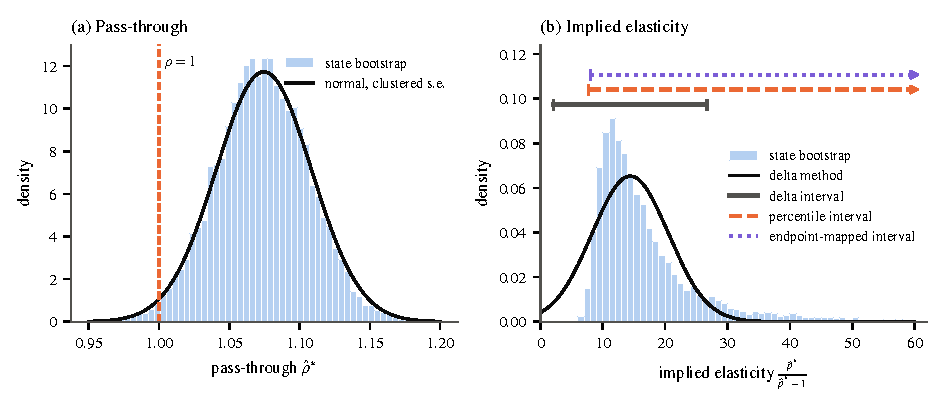
\includegraphics[width=\textwidth]{figures/appA/delta_boot.pdf}
\caption{State-cluster bootstrap of the cigarette tax pass-through regression with state and year effects. (a)
9,999 bootstrap estimates $\hat\rho^*$ and the normal density with the state-clustered standard error.
(b) Implied elasticity $\frac{\hat\rho^*}{\hat\rho^* - 1}$ and the delta-method normal density. The
horizontal bars are 95 percent intervals: delta method $[2.1, 26.7]$, bootstrap percentile $[7.7, 68.9]$, and the
mapped endpoints of the clustered interval for $\rho$, $[8.0, 162.9]$. Arrows mark intervals that extend beyond
the plotted range. 4.4 percent of the bootstrap elasticities lie outside $[0, 60]$ and are not plotted. Seed
20261022.}
\label{fig:A-delta-boot}
\end{figure}

\casehead{The Sumner panel}
We apply a pairs cluster bootstrap by state to row (1) of \cref{tab:A-sumner}, with $B = 9{,}999$. Each replication
draws 48 states with replacement, treats repeated states as distinct, and re-estimates \eqref{eq:A-sumner} with state
and year effects. The bootstrap standard error of $\hat\rho$ is 0.033, close to the clustered 0.034 and to the
jackknife value of 0.034 obtained by deleting one state at a time. \Cref{tab:A-boot-intervals} compares intervals.
For $\rho$, all methods give similar intervals that exclude one. The bootstrap distribution in
\cref{fig:A-delta-boot}(a) is close to normal, and 1.3 percent of the bootstrap estimates are at or below one.

\begin{table}[htbp]
\centering
\begin{threeparttable}
\caption{95 percent intervals for pass-through and the implied elasticity}
\label{tab:A-boot-intervals}
\small
\begin{tabular}{@{}lcc@{}}
\toprule
Method & $\rho$ & $\varepsilon = \frac{\rho}{\rho - 1}$ \\
\midrule
Clustered $t_{47}$ interval, delta method for $\varepsilon$ & $[1.006,\ 1.143]$ & $[2.1,\ 26.7]$ \\
Clustered $t_{47}$ interval, endpoints mapped & $[1.006,\ 1.143]$ & $[8.0,\ 162.9]$ \\
Bootstrap percentile & $[1.008,\ 1.137]$ & $[7.7,\ 68.9]$ \\
Bootstrap percentile for $\rho$, endpoints mapped & & $[8.3,\ 126.8]$ \\
Bootstrap basic & $[1.012,\ 1.141]$ & $[-40.1,\ 21.1]$ \\
Bootstrap percentile-$t$ & $[1.012,\ 1.143]$ & \\
Bootstrap BCa, endpoints mapped for $\varepsilon$ & $[1.012,\ 1.142]$ & $[8.0,\ 81.2]$ \\
\bottomrule
\end{tabular}
\begin{tablenotes}\footnotesize
\item Notes: Row (1) of \cref{tab:A-sumner}, $\hat\rho = 1.075$ and $\hat\varepsilon = 14.4$. Pairs cluster bootstrap
by state with 9,999 replications. The percentile-$t$ interval studentizes with the CR1 standard error in each
replication. BCa uses the jackknife over states for the acceleration ($\hat a = 0.019$, $z_0 = 0.030$).
\end{tablenotes}
\end{threeparttable}
\end{table}

For the elasticity the methods disagree sharply. Because 1.3 percent of the $\hat\rho^*$ lie below one, the same
share of bootstrap elasticities is negative and huge in magnitude. The percentile interval for $\varepsilon$ is
then not the image of the percentile interval for $\rho$. The map $\frac{\rho}{\rho - 1}$ is monotone on each side of
one, but not over the whole bootstrap support, so the transformation-respecting property fails. The basic interval
reflects the long right tail to the left and includes negative elasticities, which makes no economic sense. The
bootstrap standard deviation of the elasticity is 222, a meaningless number. The ratio has no finite moments
whenever the distribution of its denominator has positive density at zero. Intervals for $\varepsilon$ should be
built from an interval for $\rho$ and mapped through the monotone function, as in the second and last rows.

\subsection{Multi-step estimators and counterfactuals}\label{sec:A-boot-multistep}

The bootstrap's main practical advantage is that it handles estimators built in several steps. The rule is simple:
every step that uses the data must be repeated in every replication. Holding a first-step estimate fixed omits its
sampling variance, the problem that the analytical correction of \cref{prop:A-twostep} addresses. Two examples
recur in the book.

The first is a generated regressand. Marginal costs implied by a logit pricing condition, $mc_{jt} = p_{jt} -
\frac{1}{\hat\alpha(1 - S_{ft})}$, depend on the demand estimate $\hat\alpha$. Regressing them on cost shifters with
the usual standard errors treats $\hat\alpha$ as known. A market bootstrap that re-estimates $\alpha$ in each of 5,000
replications raises the standard error of the intercept from 0.016 to 0.072 in the simulated markets of
\cref{sec:C-logit-est}. The slopes barely change, because uncertainty about $\alpha$ moves all markups together.

The second is a counterfactual. \citet[WP p.~25]{ChaudhuriGoldbergJia2006} compute standard errors for counterfactual
prices and welfare losses under patent enforcement by bootstrapping the original sample 300 times. For each sample
they re-estimate the demand system and recompute the counterfactual equilibrium prices and welfare losses for each
policy scenario. When a replication's counterfactual did not converge, they compute the standard errors from the
replications that did (WP p.~25, n.~29). Dropping failed replications is common but not innocuous. If failures
occur for particular parameter values, the retained replications are a selected sample of the bootstrap distribution.

\casehead{Parametric bootstrap and parameter draws}
Two cheaper procedures are often called a parametric bootstrap, and they differ. The first simulates new data sets
from the fitted model $F(\cdot;\hat\theta)$ and re-estimates on each. It is the natural way to compute the null
distribution of a specification test whose statistic has no tractable limit. \citet[p.~241]{AtheyLevinSeira2011}
use it for the conditional Kolmogorov test of \citet{Andrews1997} and cannot reject their parametric bid model even at
the 20 percent level. The second draws parameter vectors from the estimated asymptotic distribution
$N(\hat\theta, \hat V)$ and recomputes the statistic of interest without re-estimating
(\cref{rem:A-krinsky-robb}). Athey, Levin and Seira use this second procedure for the predicted outcomes of their
Table~V (p.~248), as do \citet{Nevo2001} and \citet{Gentzkow2007}.

The validity conditions follow from what each procedure resamples. Parameter draws are valid when $\hat\theta$ is
approximately normal and $a$ is smooth. They are first-order equivalent to the delta method and cost one evaluation
of $a$ per draw. Re-estimating on resampled data also captures departures of $\hat\theta$ from normality, and it is
the only one of the three that can deliver a refinement. It is also the most expensive. \citet[p.~733,
n.~33]{Gentzkow2007} notes that bootstrapping would require estimating all parameters for each resample, which adds
greatly to the computational cost.

\subsection{When the bootstrap fails}\label{sec:A-boot-fail}

Bootstrap consistency rests on the statistic being a smooth function of the empirical distribution. Without
smoothness it can fail, and the canonical example is an extreme order statistic.

\begin{proposition}[The bootstrap of a sample maximum]\label{prop:A-boot-max}
Let $X_1, \dots, X_n$ be i.i.d.\ uniform on $[0, \theta]$ and $\hat\theta = \max_iX_i$. Then
$\frac{n(\theta - \hat\theta)}{\theta}$ converges in distribution to the standard exponential distribution, which is
continuous (\cref{prop:A-uniform-mle}). For the nonparametric bootstrap,
\begin{equation*}
  \Pr^*\bigl(\hat\theta^* = \hat\theta\bigr) = 1 - \Bigl(1 - \frac{1}{n}\Bigr)^n \longrightarrow 1 - e^{-1} \approx 0.632.
\end{equation*}
The bootstrap distribution of $\frac{n(\hat\theta - \hat\theta^*)}{\hat\theta}$ has an atom of mass about 0.632 at
zero and does not converge to the exponential limit.
\end{proposition}

\begin{proof}
The bootstrap maximum equals $\hat\theta$ if and only if the largest observation is drawn at least once. Each of the
$n$ independent draws misses it with probability $1 - \frac{1}{n}$, so it is never drawn with probability
$(1 - \frac{1}{n})^n$. Taking logs, $n\ln(1 - \frac{1}{n}) = n(-\frac{1}{n} - \frac{1}{2n^2} - \cdots) \to -1$, so
$(1 - \frac{1}{n})^n \to e^{-1}$. A limit distribution with an atom of mass $1 - e^{-1}$ at zero cannot equal the
continuous exponential distribution.
\end{proof}

The probability is already close to its limit in small samples: 0.651 for $n = 10$, 0.634 for $n = 100$ and 0.632
for $n = 1{,}000$. The intuition is that the bootstrap cannot draw values beyond the sample maximum, while the
sampling distribution of $\hat\theta$ is driven by how far the maximum falls short of the true endpoint.

The same failure appears in other non-regular problems. Parameters on the boundary of the parameter space, such as a
zero variance component, invalidate the bootstrap of the estimator \citep{Andrews2000}. Non-smooth functionals,
such as bounds formed as the maximum or minimum of estimated functions, behave like the maximum above
(\cref{sec:A-partialid}). With weak instruments the estimator is not asymptotically normal and the bootstrap does not
fix it (\cref{sec:A-weakiv}). Data with infinite variance are a further case, since the bootstrap of the sample mean
then fails. A statistic without finite moments, like the elasticity ratio above, needs a separate diagnosis. Missing
moments alone do not make the bootstrap distribution inconsistent. When the true $\rho$ is bounded away from one, the
map $\frac{\rho}{\rho - 1}$ is smooth near it. The extension of \cref{prop:A-boot-mean} to smooth functions of means
then makes the bootstrap distribution of $\sqrt n(\hat\varepsilon^* - \hat\varepsilon)$ consistent, although
$\hat\varepsilon$ has no finite moments in any finite sample. What can fail are summaries that estimate
finite-sample moments, such as the bootstrap standard deviation, because the moments they target do not exist. A true denominator at zero, or close to zero relative to its sampling error, is a
genuine non-regularity like a weak instrument. The Sumner estimate of $\rho$, about two standard errors above one, is
close to that case. Two remedies are general \citep{PolitisRomanoWolf1999}. \emph{Subsampling} recomputes the statistic on
subsamples of size $b$ drawn without replacement, with $b \to \infty$ and $\frac{b}{n} \to 0$, and rescales by the
known rate. The \emph{$m$-out-of-$n$ bootstrap} draws $m < n$ observations with replacement, with $\frac{m}{n} \to 0$.
Both work under much weaker conditions because a small subsample behaves like a fresh sample from the population.
The relevance for this book is direct. Auction models whose bid support depends on the parameters
\citep{DonaldPaarsch1996}, estimators built on extreme order statistics, and partially identified models
(\cref{ch:auction-empirics}) all fall outside the standard bootstrap's guarantees.
